%% StatsPAI -- JSS submission
%% --------------------------------------------------------------
%% Author: Biaoyue (Bryce) Wang -- brycew6m@stanford.edu
%% Class:   jss.cls (https://www.jstatsoft.org/about/submissions)
%% Compile: latexmk -pdf main.tex
%%
%% Notes
%% -----
%% * The active manuscript intentionally uses the submission-facing
%%   `\documentclass[article]{jss}` mode.  The JSS style guide reserves
%%   `nojss` for package-vignette derivatives, not for the manuscript PDF.
%% * jss.cls already provides \code, \pkg, \proglang, \email, \doi,
%%   and loads natbib (authoryear, round) + hyperref.  The earlier
%%   article-class build redefined those macros; with jss.cls they come
%%   for free and the redefinitions are intentionally dropped.
%% * The earlier article-class backup used during style migration is
%%   preserved at main-article-class.tex.bak.
%% --------------------------------------------------------------

\documentclass[article]{jss}

%% Recommended packages from the JSS template.
\usepackage{orcidlink,thumbpdf,lmodern}

%% Packages we still need beyond the JSS defaults.
\usepackage{amsmath,amssymb,amsthm}
\usepackage{booktabs,longtable,array,multirow}
\usepackage{listings}
\usepackage{enumitem}
\usepackage{microtype}
%% Printed transcripts are 20-30 lines and read badly when a page break
%% lands inside the output block; \Needspace moves the whole transcript
%% to the next page rather than splitting it.
\usepackage{needspace}

%% Code listing style approximating JSS Sinput / Soutput.  We retain
%% listings (rather than jss.cls's fancyvrb CodeInput) for the numbered,
%% cross-referenceable captions the text relies on, but the rendering is
%% deliberately verbatim-equivalent:
%%
%%   columns=fullflexible + keepspaces  -- listings' default [c]fixed mode
%%     pads every glyph into a fixed box, which spreads identifiers into
%%     "sp . datasets . card_1995 ()" in the PDF and makes the code
%%     uncopyable.  fullflexible uses the typewriter font's natural
%%     widths, so a listing sets exactly as \verb would.
%%   upquote  -- straight ' and " so a reader can paste a listing into a
%%     Python prompt without silently getting curly quotes.
%%   no language=/keywordstyle=  -- JSS does not syntax-highlight code;
%%     bolding Python keywords was a house-style deviation.
%%
%% Every printed listing is executed verbatim by
%% replication/scripts/listings_execute_audit.py, so a listing that stops
%% being runnable fails `make verify` rather than reaching a reviewer.
\definecolor{codebg}{gray}{0.96}
\lstdefinestyle{Sinput}{
  basicstyle=\ttfamily\small,
  backgroundcolor=\color{codebg},
  frame=single, framesep=4pt, framerule=0pt,
  columns=fullflexible,
  keepspaces=true,
  upquote=true,
  breaklines=true,
  breakautoindent=false,
  breakindent=2em,
  postbreak={\mbox{$\hookrightarrow$\space}},
  showstringspaces=false,
  aboveskip=1.2\medskipamount,
  belowskip=0.6\medskipamount,
}
\lstdefinestyle{Soutput}{
  style=Sinput,
  backgroundcolor=\color{codebg!60!white},
}
\lstset{style=Sinput}

%% Custom commands.  jss.cls defines \code, \pkg, \proglang for us.
%% Wrap \pkg{StatsPAI} in \texorpdfstring so the macro is also safe
%% to use inside section titles (where hyperref needs a plain-text
%% PDF-bookmark string).
\newcommand{\statspai}{\texorpdfstring{\pkg{StatsPAI}}{StatsPAI}}
%% natbib prints every author on a reference's first in-text citation.
%% For the three large-collaboration entries that means eight names and
%% two lines of body text to name one dependency, so force the
%% abbreviated form everywhere: HELM (50 authors), NumPy, SciPy, and
%% scikit-learn (16).
\shortcites{liang2023helm,harris2020array,virtanen2020scipy,%
            pedregosa2011scikit}
\newcolumntype{L}[1]{>{\raggedright\arraybackslash}p{#1}}
% AUTO-GENERATED by replication/scripts/generate_manuscript_claims.py
% Do not edit by hand; run the generator or `make manuscript-claims`.
\newcommand{\StatsPAIVersion}{1.30.1}
\newcommand{\RegistryTotal}{1{,}220}
\newcommand{\RegistryCertified}{414}
\newcommand{\RegistryValidated}{142}
\newcommand{\RegistryCertifiedValidated}{556}
\newcommand{\RegistryApiStable}{661}
\newcommand{\RegistryExperimental}{3}
\newcommand{\RegistryStableHandwritten}{274}
\newcommand{\RegistryAutoUnbacked}{568}
\newcommand{\RegistryAutoUnbackedClasslike}{292}
\newcommand{\RegistryAutoUnbackedFunctionlike}{276}
\newcommand{\RegistryOtherApiEvidence}{93}
\newcommand{\AgentCardCount}{416}
\newcommand{\AgentDefaultCardCount}{804}
\newcommand{\AgentCardPct}{34.1\%}
\newcommand{\SchemaWithTypedParameter}{1{,}188}
\newcommand{\SchemaParameterTotal}{9{,}436}
\newcommand{\SchemaParameterDescribed}{9{,}436}
\newcommand{\SchemaParameterDefault}{3{,}348}
\newcommand{\SchemaParameterEnum}{468}
\newcommand{\SchemaParameterDescribedPct}{100.0\%}
\newcommand{\SchemaParameterDefaultPct}{35.5\%}
\newcommand{\SchemaParameterEnumPct}{5.0\%}
\newcommand{\ParityCrossLanguage}{415}
\newcommand{\ParityInternalEvidence}{142}
\newcommand{\ParityEstimatorTotal}{800}
\newcommand{\ParityEstimatorCrossLanguage}{415}
\newcommand{\ParityEstimatorCrossLanguagePct}{51.9\%}
\newcommand{\ParityInfraTotal}{126}
\newcommand{\ParityClassTotal}{294}
\newcommand{\RParityModuleCount}{89}
\newcommand{\StataParityModuleCount}{85}
\newcommand{\NoStataModuleCount}{4}
\newcommand{\OrigParityModuleCount}{12}
\newcommand{\OrigParityRowCount}{35}
\newcommand{\RParityPassCount}{88}
\newcommand{\RParityNonPassCount}{1}
\newcommand{\ParityNativeModuleCount}{86}
\newcommand{\ParityPortModuleCount}{0}
\newcommand{\ParityThirdPartyModuleCount}{3}
\newcommand{\ParityBackendModuleCount}{0}


%% -- Article metainformation (JSS macros) ------------------------------------

%% Title-block affiliations are kept to two lines per author so the JSS
%% title page still holds the abstract; the full affiliation string
%% (identical to paper.md / CITATION.cff) is in \Address below.
\author{Biaoyue Wang~\orcidlink{0000-0002-1828-2208}\\
        Stanford University\\
        \emph{and} StatsPAI Inc.
        \And
        Scott Rozelle~\orcidlink{0000-0001-5053-0243}\\
        Stanford University\\
        \emph{and} StatsPAI Inc.}
\Plainauthor{Biaoyue Wang, Scott Rozelle}

\title{\statspai{}: Validation-Tiered \proglang{Python} Workflows for
       Causal Inference}
\Plaintitle{StatsPAI: Validation-Tiered Python Workflows for Causal Inference}
\Shorttitle{\statspai{}: Validation-Tiered \proglang{Python} Causal Inference}

\Abstract{
\statspai{} is a \proglang{Python} package for applied causal inference
and econometrics in which every registered function carries an evidence
tier that a user or an agent can query at call time. This article asks
what such a label certifies, and describes the design that makes the
answer checkable. Parity rows are classified by what the \statspai{}
side actually executes, verified by a call trace of every module
(\ParityNativeModuleCount{} of \RParityModuleCount{} run native code,
\ParityThirdPartyModuleCount{} wrap third-party \proglang{Python}
libraries, and none call the reference they are compared against);
evidence is recorded per configuration, so a user can ask whether the
variant, inference option, and code path just fitted is the one that was
tested; automated diagnostics distinguish a missing check from one that
does not exist for the fit; and stochastic estimators are graded by
seed-replicated equivalence against an explicit margin rather than by
their sampling standard errors. The evidence covers a twelve-estimator
core: same-byte parity with canonical \proglang{R} implementations
(\RParityModuleCount{} modules) and audited \proglang{Stata} bridges
(\StataParityModuleCount{}), known-truth recovery, Monte Carlo coverage
at \(B=1{,}000\) reported with bias, Monte Carlo standard deviation, and
standard-error calibration, and a performance study that keeps
unfavourable comparisons. Applying the design to the package found
defects that numerical agreement alone had not: two parity rows that
compared \proglang{R} with itself, a coverage row that measured a
different estimator from the one it named, an entropy-balancing standard
error twice the estimator's Monte Carlo standard deviation, and an audit
that requested an over-identification test for a just-identified model.
Seven worked examples, executed verbatim and one returning the same numbers as its
\proglang{R} and \proglang{Stata} references on identical bytes, and a
licence-free replication path complete the article. The evidence for
the agent-facing interface is mechanical and contractual, not a claim of
behavioural agent superiority.
}

\Keywords{causal inference, applied econometrics, validation tiers, \proglang{Python},
          \proglang{R}, \proglang{Stata}, software, machine learning,
          agent-facing registry API, large language models, reproducibility}
\Plainkeywords{causal inference, applied econometrics, validation tiers, Python, R,
               Stata, software, machine learning, agent-facing registry API,
               large language models, reproducibility}

\Address{
  Biaoyue Wang (corresponding author)\\
  Rural Education Action Program, Stanford Center on China's Economy and Institutions,\\
  Stanford University, United States\\
  \emph{and} StatsPAI Inc., United States\\
  E-mail: \email{brycew6m@gmail.com}, \email{brycew6m@stanford.edu}\\
  URL: \url{https://github.com/brycewang-stanford/StatsPAI}\\[6pt]
  Scott Rozelle\\
  Rural Education Action Program, Stanford Center on China's Economy and Institutions,\\
  Stanford University, United States\\
  \emph{and} StatsPAI Inc., United States\\
  E-mail: \email{rozelle@stanford.edu}
}

\begin{document}

\section{Introduction}\label{sec:intro}

Applied causal work now spans a large and fragmented software stack:
\proglang{Stata} commands, methodological-reference \proglang{R}
packages, and an expanding but incomplete \proglang{Python} ecosystem.
A single project can require OLS and IV, staggered
difference-in-differences, regression discontinuity, synthetic control,
matching, double machine learning, sensitivity analysis, and publication
tables. The statistical literature has converged toward more explicit
design checks and estimator-specific inference
\citep{imbens2009recent,angrist2009mostly,callaway2021difference,
roth2023whats,wing2024designing,baker2026difference,rambachan2023more,abadie2010synthetic,
chernozhukov2018double}; the software interface has not converged with
it. Users still cross package boundaries, result classes, naming
conventions, and diagnostic vocabularies. Large-language-model agents
add a further constraint: they need typed schemas and structured errors,
not prose-only help pages.

This paper introduces \statspai{}, a \proglang{Python} platform for
applied econometrics and causal inference. The package provides
(i) a unified \code{import statspai as sp} surface across common causal
designs, (ii) shared reporting conventions for mature estimator results,
diagnostics, citations, and export methods, (iii) a machine-readable registry that can be exposed through a
Model Context Protocol (MCP) server~\citep{anthropic2024mcp}, and (iv) an explicit validation
discipline against analytical targets, canonical \proglang{R}
implementations, and selected \proglang{Stata} migration bridges. This article describes \statspai{} \StatsPAIVersion{}, distributed on PyPI
(\code{pip install statspai}, tag \code{v\StatsPAIVersion{}}) under the MIT
licence, with source at
\url{https://github.com/brycewang-stanford/StatsPAI}.

A short paper on the package appeared in the \emph{Journal of Open
Source Software}~\citep{wang2026statspaijoss}. It established the
unified interface, the registry and agent schemas, the structured result
objects, and the existence of a same-byte cross-language parity harness
and of a 1{,}000-replication coverage run for OLS, DiD, and IV. This
article does not re-establish those facts. Its question is the one a
parity harness raises but cannot answer by itself: \emph{what exactly
does a validation label certify?} A green parity row can be earned by
the wrong code (a \proglang{Python} wrapper that calls the \proglang{R}
reference it is compared against), vouch for the wrong function (an
alias credited with evidence that ran another entry point), rest on the
wrong statistical comparison (a stochastic estimator judged against its
sampling standard error rather than its own Monte Carlo error), or
describe a configuration the user is not running. The contribution is
the design that makes those failure modes checkable, and the evidence
of what applying it found. Concretely, the article adds (i) evidence
provenance that is verified rather than asserted --- every parity row is
classified by what the \statspai{} side actually executes, checked by
a call trace, and every inherited label must name a test that ran the
inheriting function (Sections~\ref{sec:track-a}
and~\ref{sec:attachment-audit}); (ii) statistical-applicability
semantics for automated diagnostics, so that a check which does not
exist for a fit is reported as not applicable rather than missing
(Section~\ref{sec:ex-card}); (iii) a seed-replicated standard for
stochastic estimators that separates algorithmic Monte Carlo error from
sampling error and states equivalence against an explicit margin
(Section~\ref{sec:validation-tiers}); (iv) a fixed adjudication procedure
for disagreements, with its outcomes (Section~\ref{sec:adjudication});
and (v) new evidence the JOSS paper does not contain: the estimand and
identification contracts of a twelve-estimator core, configuration-level
coverage diagnostics (bias, Monte Carlo SD, standard-error calibration,
interval length), a performance study that reports unfavourable
comparisons, and seven executed worked examples. Applying the design to
its own package found defects that numerical parity alone had not: two
Honest-DiD rows that compared \proglang{R} with itself, a causal-forest
coverage row whose entry point reported a separate AIPW estimator rather
than the forest's, an entropy-balancing standard error twice the
estimator's Monte Carlo SD, and an audit that asked for an
over-identification test on a just-identified model.
The registry distinguishes \code{certified}, \code{validated},
\code{api\_stable}, and \code{experimental} symbols -- queryable at
call time -- so numerical validation is an
evidence tier rather than a blanket claim over the whole API surface;
the full census opens Section~\ref{sec:parity}.

Listing~\ref{lst:motivating} fixes ideas. The classical
\citet{card1995using} returns-to-schooling design is estimated four
ways --- OLS, instrumental variables, double machine learning
\citep{chernozhukov2018double}, and a causal forest
\citep{wager2018estimation} --- from a single import, and three of the
four fitted objects, which belong to three different result classes,
are rendered into one publication table by a single call.
Three design properties recur throughout the paper: the
estimator surface is \emph{flat} (classical and modern methods are
siblings under \code{sp.}); the result objects are \emph{interoperable}
(mixed estimators feed directly into one \code{sp.regtable} call); and
the platform exposes \emph{audit hooks} (\code{sp.audit}) that list
the diagnostic evidence a design demands but the user has not yet
supplied. Section~\ref{sec:ex-card} runs the same session at a prompt
and prints what each of these calls returns.

Every listing in this paper is executed verbatim by the replication
archive's listing audit, and for the transcripts the audit goes
further: it replays each one statement by statement through a real
interpreter loop and compares the output printed here, line for line,
with the output the code actually produces
(Section~\ref{sec:reproducibility}). A printed transcript is quoted as
evidence and read as evidence, so it is checked like evidence.

\begin{lstlisting}[caption={\statspai{} reproduces and extends Card
(1995) from a single import; classical and modern estimators are
siblings under \code{sp.} and return one interoperable result
contract.},label={lst:motivating},captionpos=b]
import statspai as sp

card = sp.datasets.card_1995()
X    = ["exper", "expersq", "black", "south", "smsa"]

ols = sp.regress("lwage ~ educ + " + " + ".join(X), data=card)
iv  = sp.iv("lwage ~ " + " + ".join(X) + " + (educ ~ nearc4)",
            data=card)
dml = sp.dml(card, y="lwage", d="educ", X=X,
             model="plr", n_folds=5, random_state=42)
cf  = sp.causal_forest("lwage ~ educ | " + " + ".join(X), data=card,
                       n_estimators=2000, discrete_treatment=False,
                       random_state=42)

table = sp.regtable(ols, iv, dml, keep=["educ", "ATE"], stars=True,
                    model_labels=["OLS", "2SLS", "DML PLR"])
table.to_docx("returns_to_schooling.docx")
\end{lstlisting}

The package surface is deliberately broad, spanning classical
regression and panel models, the modern DiD, RD, and synthetic-control
literatures, ML-based treatment-effect estimation, matching and
weighting, sensitivity analysis, and publication output.
Breadth, however, is not the paper's evidentiary claim.
In this paper, ``validated'' means a
specific artifact exists: known-truth recovery, cross-language parity on
identical data bytes, Monte Carlo coverage, or an explicit convention
disclosure. Unit and regression tests are API-contract evidence; they
do not by themselves promote a helper into the numerical-validation
tier. An \code{api\_stable} helper has a stable call signature; it does
not acquire statistical credibility by proximity to validated estimators.
Table~\ref{tab:scope} makes this boundary explicit before the paper
turns to architecture and validation evidence.

\begin{table}[!ht]
\centering\scriptsize
\begin{tabular}{p{0.23\linewidth}p{0.36\linewidth}p{0.31\linewidth}}
\toprule
Layer & Examples & Evidence used in this paper \\
\midrule
Unified causal API & OLS/IV, DiD, RD, synth, DML, forests, matching,
causal-impact workflows & Shared entry points, mature result objects, exports,
and worked examples \\
Validated causal core & The twelve-estimator validation suite
& Analytical recovery, R parity, selected Stata bridges, coverage, and
performance checks \\
Agent-facing surface & Registry schemas, agent cards, MCP tools,
structured errors & Schema coverage, deterministic MCP trace, and
citation/audit checks \\
Broader registry & Long-tail econometric helpers and optional backends
& Reported as \code{api\_stable} or \code{experimental} unless backed by
the same evidence standard \\
\bottomrule
\end{tabular}
\caption{Scope of the submission. The package is broader than the
validated core; the paper-level claim is limited to the rows backed by
the artifacts in Sections~\ref{sec:examples}--\ref{sec:agentbench}.}
\label{tab:scope}
\end{table}

The closest implementations cover important parts of this terrain, but
with different centers of gravity; Table~\ref{tab:related-software}
states the comparison directly. Empirical comparisons appear later in
the same-byte parity rows
(Tables~\ref{tab:track-a-cross-language-snapshot}
and \ref{tab:headline-parity}) and in the timing study
(Figure~\ref{fig:track-c-loglog}); per-entry-point detail is generated
into \path{Paper-JSS/parity/replacement-table.md}. The contribution is therefore an
integration-and-validation layer around reference software, not a claim
that \statspai{} supersedes specialized packages or reference
implementations in their home domains, such as
\pkg{fixest}, \pkg{did}, \pkg{rdrobust}, \pkg{Synth},
\pkg{synthdid}, \pkg{DoubleML}, or \pkg{grf}. Representative software
citations include \pkg{Synth}, \pkg{MatchIt}, \pkg{DoubleML},
\pkg{EconML}, \pkg{CausalML}, and \pkg{DoWhy}
\citep{abadie2011synth,ho2011matchit,bach2022doubleml,econml,
chen2020causalml,sharma2020dowhy}.

\begin{table}[!ht]
\centering\scriptsize
\begin{tabular}{p{0.23\linewidth}p{0.32\linewidth}p{0.35\linewidth}}
\toprule
Comparable implementation & Where it remains the reference choice & \statspai{} contribution and boundary \\
\midrule
\pkg{statsmodels}, \pkg{linearmodels}, \pkg{pyfixest} &
Mature regression, panel, covariance, and HDFE APIs with focused
maintainer communities. &
\statspai{} adds a causal-workflow layer, audit prompts, citations, and
agent schemas around common calls; it is not a replacement for their
full model-specific APIs or fastest specialist paths. \\
\pkg{DoubleML}, \pkg{EconML}, \pkg{CausalML}, \pkg{grf} &
Deeper ML-causal and CATE-specific surfaces, tuning controls, and
method-family specialization. &
\statspai{} places DML and forests inside the same result, audit, and
validation ledger; the forest row is only a T3 stochastic agreement
claim, not deterministic parity with every \pkg{grf} option. \\
\pkg{DoWhy} &
Graph-first identification and refutation workflows. &
\statspai{} is estimator- and evidence-led: it emphasizes parity
artifacts and shared output contracts, but it does not attempt to match
graph-identification automation. \\
\pkg{did}, \pkg{fixest}, \pkg{rdrobust}, \pkg{rddensity},
\pkg{Synth}, \pkg{synthdid}, \pkg{MatchIt}, and Stata commands such
as \code{csdid}, \code{reghdfe}, \code{rdrobust}, and \code{sdid} &
Authoritative reference implementations in their home ecosystems,
often with more mature edge-case options and community history. &
\statspai{} validates against these references on identical data bytes
where possible and records disagreements as ledger entries rather than
strict parity claims; the remaining T4 disclosure is the classical-SCM
identification/non-uniqueness gap on the calibrated Basque replica,
while generalized SCM, RD-density,
and SDID are native parity rows in \StatsPAIVersion{}. Stata bridges require
a separate licensed runtime. \\
\pkg{differences}, \pkg{causalimpact}, and narrower workflow packages &
Focused workflows with less surface area for users who need exactly
that model family. &
\statspai{} standardizes cross-family handoffs through one namespace
and one post-estimation contract; that breadth comes with a larger
dependency surface and a validation ledger that should be read row by
row. \\
\bottomrule
\end{tabular}
\caption{Closest existing implementations and comparative scope,
surveyed in May 2026 and spot-checked in September 2026.}
\label{tab:related-software}
\end{table}

The submission should therefore be read in three layers. The manuscript
describes the user-facing API and the statistical-software design
choices; the validation tables state which methods have parity,
coverage, performance, or boundary evidence; and the replication archive
contains the executable ledgers that determine whether a label such as
\code{certified}, \code{validated}, or \code{api\_stable} is justified.
This separation is intentionally conservative: a broad namespace is
useful only if readers can tell which parts are statistical evidence and
which parts are stable software infrastructure.
To keep the printed article compact, the archive also includes a
reviewer evidence map and editor screening checklist that route
validation-scope, reproduction, related-review and COI, sustainability,
and release-boundary questions to executable artifacts.

Section~\ref{sec:architecture} describes the architecture the evidence
attaches to and Section~\ref{sec:agent} the agent-facing interface;
Section~\ref{sec:examples} runs seven worked examples, with staggered
DiD as the main case study; Sections~\ref{sec:parity}--\ref{sec:agentbench}
report the validation, performance, and interface evidence.

\section{Software architecture}\label{sec:architecture}

\statspai{} is implemented in \proglang{Python} on top of
\pkg{NumPy} \citep{harris2020array}, \pkg{SciPy}
\citep{virtanen2020scipy}, \pkg{pandas} \citep{mckinney2010data},
\pkg{statsmodels} \citep{seabold2010statsmodels}, \pkg{scikit-learn}
\citep{pedregosa2011scikit}, and \pkg{linearmodels}, with optional
backends kept behind extras and lazy imports. The architecture has four layers:
registry, dispatcher, result object, and output pipeline.

\subsection{Design principles}\label{sec:design-principles}

Seven principles govern the public API. A single flat namespace exposes
routine calls through \code{sp.<function>}. Mature estimator paths return
structured result objects rather than raw tuples, while auxiliary
helpers -- visualization and data-inspection utilities such as
\code{sp.panel\_view}, which returns Matplotlib handles plus an
\code{info} dictionary rather than an estimator result -- remain
registered with explicit stability and validation
metadata. Method families use dispatchers
(\code{sp.synth(method=...)}, \code{sp.dml(model=...)},
\code{sp.did(...)}). Reference parity is
attempted before broadening a validated claim. Failures are loud:
assumption violations raise typed exceptions or warnings and record
diagnostics. Output-changing changes go through the changelog and
\code{MIGRATION.md}. Finally, every public function must be
discoverable through the same registry used by human help functions and
agent schemas.

\subsection{Why an integration package?}\label{sec:why-integration}

A reasonable alternative is to compose \pkg{statsmodels},
\pkg{linearmodels}, \pkg{DoubleML}, \pkg{EconML}, \pkg{DoWhy}, and
method-specific \proglang{R} or \proglang{Stata} bridges directly,
which is often right for a single specialized model. The friction
appears when an applied project moves across identification designs:
diagnostics, citations, validation status, error handling, export
formats, and agent schemas no longer share one contract. \statspai{}
therefore treats wrapping as insufficient unless a method enters the
common registry, result-object surface, typed-error envelope, and
evidence ledger. Specialized packages remain the reference
implementations; the contribution here is to make cross-family handoffs
auditable and reproducible. The package is organized by identification
layer rather than by the historical boundaries of \proglang{R} and
\proglang{Stata} packages -- each layer reports its own design
diagnostics (balance and overlap, first-stage strength, cohort support
and event-study paths, bandwidth and density checks, donor weights and
placebos, cross-fit diagnostics) -- and the common point is not shared
identification assumptions but a shared post-estimation contract.

\subsection{Registry and discovery layer}\label{sec:registry}

The central data structure is a registry of \code{FunctionSpec}
records. Each entry carries a canonical function path, category, tags,
stability and validation status, parameter metadata, result class,
reference key, example call, and optional agent-card fields such as
assumptions, preconditions, failure modes, alternatives, limitations,
and typical sample-size guidance. The registry powers
\code{sp.help()}, \code{sp.list\_functions()},
\code{sp.search\_functions()}, \code{sp.describe\_function()},
\code{sp.function\_schema()}, \code{sp.agent\_card()}, the import-free
\code{schemas/} bundle, and the MCP tool catalogue. Tests assert that
exported public callables are registered and that validated/certified
entries expose their evidence status.

The validation tier is therefore not a paper-only artifact: it is
queryable from the running software for \emph{every} registered
function. \code{sp.help()} prints a per-tier census and points the user
to \code{sp.list\_functions(validation\_status="certified")} for the
validated core, while \code{sp.describe\_function(name)} prints a
\code{Stability}/\code{Validation} header with the attached evidence
notes before the description, so a user or agent landing on an
\code{api\_stable} or \code{experimental} helper sees its trust tier
before relying on its output.

\begin{lstlisting}[caption={The validation tier is visible through the
same discovery surface used by users and agents; this excerpt is
generated from \code{sp.describe\_function("callaway\_santanna")}.},%
label={lst:validation-tier-output},captionpos=b]
>>> spec = sp.describe_function("callaway_santanna")
>>> spec["stability"], spec["validation_status"]
('stable', 'certified')
>>> for note in spec["validation_notes"][:3]:
...     print(note)
Track A parity seed
R parity module 04_csdid
Stata parity module 04_csdid
>>> import textwrap
>>> print(textwrap.fill(spec["limitations"][0], width=64))
clustervars is not yet supported with bstrap=False; the analytic
standard errors do not account for within-cluster dependence, so
the multiplier bootstrap is required
\end{lstlisting}

\subsection{Family dispatchers}\label{sec:dispatcher}

Family dispatchers reduce method sprawl without hiding assumptions.
\code{sp.synth} dispatches classical, SDID, augmented, generalized,
matrix-completion, penalized, and related synthetic-control variants.
\code{sp.decompose} covers Blinder--Oaxaca, Gelbach, Fairlie, RIF,
DFL, Machado--Mata, Melly, counterfactual-distribution, and related
decompositions. \code{sp.dml} dispatches partially-linear,
partially-linear IV, interactive, and LATE-style DML variants. The
dispatcher contract is explicit: allowed \code{method=} values are
enumerated in the registry schema, and validated or mature variants
return compatible result surfaces so that summary, plotting, audit,
citation, and export calls do not change downstream.

The same uniformity extends to inference. Across the regression family
(\code{regress}, \code{feols}, \code{ivreg}, \code{panel},
\code{hdfe\_ols}), one canonical keyword, \code{vce=}, spells the full
standard-error menu: classical, heteroskedasticity-robust, one- and
two-way clustering, bias-reduced CR2/CR3
\citep{pustejovsky2018small}, the wild cluster bootstrap
\citep{cameron2008bootstrap, roodman2019fast}, and Conley spatial HAC
\citep{conley1999estimation}; fixed-effects Poisson and GLM
additionally expose CR2/CR3 and the restricted score wild bootstrap.
Each option is pinned to an external reference implementation ---
\proglang{Stata}'s \code{reghdfe}, \code{boottest}, \code{acreg}, and
\code{ppmlhdfe} \citep{correia2020fast}, and \proglang{R}'s
\pkg{clubSandwich} and
\pkg{sandwich} \citep{zeileis2020sandwich} --- and a coverage matrix in the package's continuous
integration ratchets the count of natively wired, externally validated
cells monotonically upward.

\subsection{Result-object hierarchy}\label{sec:results}

Most estimators return either \code{EconometricResults} or
\code{CausalResult}; specialized classes must implement the same public
surface. The standard contract covers summaries, plotting, dictionary
and JSON payloads, LaTeX/DOCX export, citations, audits, diagnostics,
and degradation records. This is why a mixed OLS/IV/DML/forest
table can be passed to \code{sp.regtable} (or its \proglang{R}-style
alias \code{sp.modelsummary}), and
why an MCP agent can keep only a result handle rather than copying
coefficient and covariance arrays between tool calls.

\subsection{Performance backbone}\label{sec:perfbackbone}

The performance-critical path is high-dimensional fixed-effect
absorption for fixed-effect and panel estimators. The submitted artifact
uses the reproducible \proglang{Python} path built on \pkg{NumPy} and
\pkg{Numba} \citep{lam2015numba}. An experimental Rust crate and selected \pkg{JAX} and
\pkg{PyTorch} paths exist behind extras, but the numerical and timing
claims in this paper do not depend on a compiled native extension.
Optional acceleration is treated as a backend choice, not as a separate
estimator or a hidden requirement.

\subsection{Output pipeline}\label{sec:output}

Publication output is unified through \code{sp.regtable},
\code{sp.modelsummary}, and result-level exporters. Mixed
\code{EconometricResults} and \code{CausalResult} objects can be
rendered as LaTeX, Markdown, HTML, Word, Excel, or JSON-safe agent
payloads. \code{sp.outreg2} gives a Stata-like migration surface, while
\code{sp.paper()} uses the same rendering layer to assemble tables,
figures, citations, and a report.

\subsection{The four-stage workflow}\label{sec:workflow}

The layers combine into a four-stage workflow -- detect
(\code{sp.detect\_design}, \code{sp.preflight}, \code{sp.recommend}),
fit (the estimator dispatchers), inspect (\code{summary()},
\code{plot()}, \code{sp.audit()}, sensitivity wrappers), and report
(\code{sp.regtable}, export methods, \code{cite()},
\code{sp.paper()}) -- with the same
boundaries available to human users and to MCP agents.

\section{The agent-facing registry API}\label{sec:agent}

\statspai{} exposes the same surface used by a human Python user to
LLM agents through typed schemas and an MCP server. The paper's claim is
mechanical and contractual: schemas, typed errors, result handles,
citations, and deterministic traces make machine-orchestrated calls
inspectable by the same validation ledger as human calls. It is not a
behavioural claim that an autonomous agent will always choose the right
empirical design. The agent layer is a software-interface contribution
rather than an intelligence benchmark: it reduces four otherwise opaque
handoffs -- tool discovery, failure recovery, result reuse, and citation
resolution -- to artifacts a reviewer can inspect in the same archive,
which is why the validation target is schema/MCP/citation
reproducibility, not a model-quality score.

\subsection{Why a schema, not a docstring}\label{sec:why-schema}

Docstrings, \proglang{R} help pages, and \proglang{Stata} help files are
prose interfaces. A tool-using agent needs a typed object containing
parameter names, types, defaults, required fields, enumerated choices,
and a short description including stability and limitations when
relevant. The schema call returns the executable OpenAI-style object;
the description and agent-card calls return richer planning metadata
such as assumptions, preconditions, failure modes, alternatives, typical
sample size, references, and examples.

\subsection{The function-schema layer}\label{sec:fn-schema}

The discovery surface lists registered functions, describes a selected
function, emits its executable schema, and returns curated agent cards.
These functions are themselves registered, which lets an agent inspect
the available estimator catalogue before selecting a method.
Complementary design-detection and preflight calls expose cheap planning
diagnostics before an estimator is run.

\subsection{The typed exception envelope}\label{sec:exception-envelope}

Estimator failures inherit from \code{StatsPAIError} and carry
structured fields: \code{error\_kind}, \code{detail},
\code{recovery\_hint}, \code{alternative\_functions}, and any partial
\code{diagnostics}. Warnings use the same idea for non-fatal
degradations. The MCP server serializes these records as structured
errors, so an agent can branch on \code{weak\_instrument},
\code{no\_overlap}, \code{rank\_deficient}, or similar identifiers
without scraping English messages.

\subsection{The estimand-first DSL and robustness audit}\label{sec:causal-question}

\code{sp.causal\_question(...)} accepts a requested estimand, treatment,
outcome, data, optional design, covariates, instruments, and sensitivity
flag, then routes to the appropriate estimator and returns a
\code{CausalQuestionResult}. The result bundles the fitted estimator,
the design-detection provenance, optional sensitivity output, and an
\code{audit\_report}. The standalone \code{sp.audit(result)} call
produces the same missing-evidence checklist for any fitted result and
points to follow-up functions such as RD density tests, Honest-DiD
sensitivity, or unobserved-confounding bounds. Each check carries one of
four statuses --- passed, failed, missing, or not applicable --- and the
last is decided from the fit's own metadata by an explicit
applicability rule (an over-identification test is not applicable to a
just-identified IV model, and says why), so an agent is never sent after
a test that does not exist. The companion \code{sp.validation\_scope}
answers the neighbouring question of which validation artifacts cover
the fitted configuration (Section~\ref{sec:validation-tiers}).

\subsection{The bibliography verifier}\label{sec:cite}

Every public-facing citation emitted by the package must come from the
curated \code{paper.bib}. Function specs store bibliography keys, result
objects expose \code{cite(format=...)}, and tests assert that registered
keys parse cleanly and do not collide on author/year/title triples.
When a key is missing, the package raises an error rather than emitting
a plausible-looking citation. This targets a concrete agent failure
mode: hallucinated references.

\subsection{The MCP server}\label{sec:mcp}

The \code{statspai-mcp} server exposes registered functions as MCP
tools. Tool inputs are generated from the registry schemas, outputs are
JSON-safe result payloads plus \code{result\_id} handles, and typed
errors use the exception envelope above. Chained tools cover auditing,
Honest-DiD sensitivity, generic sensitivity analysis, CS aggregation,
Bacon decomposition, paper generation, and citation, and they accept
result handles instead of requiring an agent to marshal coefficient,
covariance, or cross-fit arrays through model context. The
deterministic trace in Section~\ref{sec:agentbench} exercises this
contract.

\subsection{Comparison with existing platforms and prior art}\label{sec:agent-compare}

Generating a JSON schema from a typed signature is solved by
\pkg{Pydantic}, \pkg{FastAPI}, and the LLM-vendor tool adapters; what
is package-specific here is that the
schema is the statistical registry itself, tied to validation status
and typed statistical errors, with result handles for
estimate-to-audit-to-sensitivity chains -- a validation-tiered tool
catalogue with a citation verifier, which statistical help systems do
not expose.

\section{Worked examples}\label{sec:examples}

The paper uses seven worked examples as an end-to-end smoke test of the
validated core rather than as seven miniature empirical papers. Each
example has an executable script under \code{Paper-JSS/replication/}
that writes JSON, table fragments, and any figures used by the build.
The examples cover the identification strategies an applied
econometrician is most likely to ask a unified \proglang{Python}
front end to handle: selection on observables, IV, staggered DiD, RD,
synthetic control, machine-learning treatment-effect estimation,
matching, causal time-series counterfactuals, and -- the case that
reaches across all three ecosystems -- panel counterfactual estimators
and interaction effects run on the same bytes in \proglang{Python},
\proglang{R}, and \proglang{Stata}.

The non-trivial workflow case study is the \code{mpdta} staggered-DiD
example: it moves from design-specific estimation to aggregation,
event-study inspection, Honest-DiD sensitivity, Bacon decomposition,
citations, and export from the same fitted objects. The other examples
are shorter stress tests around the same contract, especially where a
reference package, public data extract, or known-truth simulation gives a
clean validation target.
Table~\ref{tab:worked-example-map} maps those examples to the
replication scripts and validation facts used by the paper.

\begin{table}[!ht]
\centering\scriptsize
\begingroup
\setlength{\tabcolsep}{3pt}
\begin{tabular}{@{}p{0.16\linewidth}p{0.20\linewidth}p{0.27\linewidth}p{0.23\linewidth}@{}}
\toprule
Example & \statspai{} surface exercised & Headline validation fact & Replication artifact \\
\midrule
Card (1995) & \code{sp.regress}, \code{sp.iv}, \code{sp.dml}, forest &
OLS and 2SLS match \proglang{R} on \code{wooldridge::card} at machine precision; DML/forest are reported as stochastic ML checks. &
\code{ex01\_card.py}; original-data module \code{01\_card} \\
Basque (2003) & \code{sp.synth}, sensitivity &
ADH special-predictor specification on the original bytes gives post-1970 gap \(-0.8946\) vs \proglang{R} \(-0.8944\) vs \proglang{Stata} \(-0.8943\); default \(V\)-choice is disclosed separately. &
\code{ex02\_basque.py}; original-data module \code{03\_basque} \\
\texttt{mpdta} staggered DiD & CS, aggregation, Honest-DiD, Bacon &
Simple ATT matches \pkg{did} and \code{csdid} to machine precision on the calibrated replica bytes, and matches \pkg{did} at \(2.3\times10^{-14}\) on the original \code{did::mpdta} bytes. &
\code{ex03\_csdid.py}; module \code{04\_csdid} \\
Lee (2008) RD & RD robust and density diagnostics &
The native CCT bandwidth and robust estimate match \pkg{rdrobust} on the RDsenate extract to \(3\times10^{-13}\); the official \pkg{rdrobust} \proglang{Python} port agrees with the native path. &
\code{ex04\_lee.py}; modules \code{06\_rd}, \code{09\_rddensity} \\
LaLonde / Dehejia--Wahba & OLS, PSM, IPW, balance diagnostics &
Original public extracts from \pkg{MatchIt} and \pkg{causalsens} match \proglang{R}; the observational design preserves the classic sign/bias warning. &
\code{ex05\_lalonde.py}; original-data modules \code{04}, \code{04b} \\
Advertising lift & \code{sp.causal\_impact} &
Known simulated lift \(=4.2\) is recovered at \(4.306\) with the 95\% interval containing truth and pre-period RMSE below the registered guard. &
\code{ex06\_causal\_impact.py} \\
fect / interflex & \code{sp.panel\_view}, \code{sp.fect}, \code{sp.interflex} &
Three fect outcome models and three interflex estimators return the same numbers as \proglang{R} \pkg{fect} / \pkg{interflex} and the authors' \proglang{Stata} commands on identical bytes (worst relative gap \(10^{-9}\)). &
\code{ex08\_fect\_interflex.py}; modules \code{86\_fect}, \code{87\_interflex} \\
\bottomrule
\end{tabular}
\endgroup
\caption{Worked-example coverage and replication artifacts. Each row is
reproduced by the named script under \code{Paper-JSS/replication/}; the
main text keeps to the executable contract and the headline validation
fact, while full per-row provenance lives in the replication archive.}
\label{tab:worked-example-map}
\end{table}

\subsection{Card (1995): returns to schooling}\label{sec:ex-card}

The Card workflow \citep{card1995using} loads the NLSYM extract, fits
OLS, 2SLS, DML, and a causal forest through the same
\code{(y, X, data)} contract, and exports the resulting table with
\code{sp.regtable}. \code{sp.datasets.card\_1995()} returns the public
\code{wooldridge::card} extract itself, so the session of
Listing~\ref{lst:motivating} runs on the original bytes;
Listing~\ref{lst:card-output} continues that session at a prompt and
prints what it produces.

\Needspace*{30\baselineskip}
\begin{lstlisting}[caption={The session of
Listing~\ref{lst:motivating}, continued at a prompt: three result
classes render into one table, and \code{sp.audit} separates the checks
this fit has passed, still lacks, or cannot have. Printed with
\code{rules="ascii"} so the transcript is byte-safe on any console
code page.},label={lst:card-output},captionpos=b]
>>> print(sp.regtable(ols, iv, dml, keep=["educ", "ATE"], stars=True,
...                   model_labels=["OLS", "2SLS", "DML PLR"],
...                   rules="ascii"))
==============================================================
                             OLS          2SLS       DML PLR
==============================================================
educ                   0.0740***     0.1323***
                        (0.0035)      (0.0492)

ATE                                                0.0741***
                                                    (0.0037)

==============================================================
First-stage F                            16.72
==============================================================
N                          3,010         3,010         3,010
R2                         0.291         0.225
Adj. R2                    0.289
F                        204.932
==============================================================
Standard errors in parentheses
*** p<0.01, ** p<0.05, * p<0.10
>>> print(sp.audit(iv))
Reviewer audit: IV-2SLS [iv]
1 of 2 applicable checks satisfied (passed 1, failed 0, missing 1; 1 n/a)

  passed  weak_instrument         value 16.72 vs threshold 10
  n/a     overid_test             just-identified; no restriction to test
  missing anderson_rubin_ci       run sp.anderson_rubin_ci

Missing checks are evidence a reviewer will expect, not errors.
n/a checks do not exist for this fit and are not counted.
\end{lstlisting}

The three linear-in-\code{educ} summaries land where the literature
puts them: \(\hat\beta_{\mathrm{OLS}} = 0.07401\) against Card's
published 0.075, and
\(\hat\beta_{\mathrm{IV}}^{\mathrm{nearc4}} = 0.1323\) against his
0.132, reproducing the IV-above-OLS pattern that motivates the design;
cross-fit DML agrees with OLS to the third decimal. \proglang{R}'s
\code{lm}+\pkg{sandwich} and \pkg{AER}\code{::ivreg} return the same
two coefficients on the same CSV bytes at relative errors
\(7.9\times 10^{-15}\) and \(1.6\times 10^{-11}\)
(Table~\ref{tab:headline-parity}). The \code{sp.audit} block is the
audit-hook claim made concrete, and it distinguishes three states that a
flat checklist conflates. The first-stage \(F\) of 16.72 clears the
\(F>10\) rule of thumb \citep{staiger1997instrumental,stock2005testing};
``passed'' means only that this screen was met --- it is neither a test
of instrument validity nor a guarantee against weak-instrument
distortion, which is why weak-instrument-robust Anderson--Rubin inference
is still listed as missing. The over-identification test is reported as
not applicable rather than missing: with one endogenous regressor and one
excluded instrument the model is just-identified, the Sargan/Hansen
statistic has zero degrees of freedom, and there is no restriction to
test. The audit reads the instrument and endogenous-regressor counts from
the fitted object to decide this; when an over-identified fit already
carries a \(J\) statistic it is read and graded, and the text, JSON, and
MCP outputs carry the same \code{not\_applicable} status and reason.

The four estimators do not share one identification argument, and the
table should not be read as four estimates of one parameter. The 2SLS
coefficient uses \code{nearc4} as an excluded instrument and, with
heterogeneous returns, identifies a local average effect for
instrument-compliers under relevance, exclusion, independence, and
monotonicity. The DML and forest calls in Listing~\ref{lst:motivating}
use no instrument: they adjust for the listed covariates and are causal
only under conditional exogeneity of schooling, the assumption the IV
design exists to avoid. On these data they therefore estimate an
adjusted partial association, and the forest's heterogeneity is
heterogeneity in that association. The listing shows that the four fits
share one result contract; it does not identify heterogeneous returns to
schooling, which would require an IV-based heterogeneity estimator and
its own validation. With that caveat, Listing~\ref{lst:card-cate}
summarises the fitted forest's conditional effects.

\Needspace*{14\baselineskip}
\begin{lstlisting}[caption={How far the return to schooling varies
across the sample, from the forest fitted in
Listing~\ref{lst:motivating}. With \pkg{grf}'s honest, 2{,}000-tree
defaults the interquartile range spans roughly 6.3\% to 8.6\% per year
around a mean of 7.7\%, as \proglang{R} \pkg{grf} finds on the same
bytes (6.3\% to 8.7\% around 7.6\%): the estimated dispersion is
modest, about a fifth of the 0.081 standard deviation the pre-1.29.0
forest engine reported for the same call on the same
data.},label={lst:card-cate},captionpos=b]
>>> print(sp.cate_summary(cf).loc[["Mean (ATE)", "Std. Dev.",
...                                "Q25", "Q75"]].round(4))
              CATE
Mean (ATE)  0.0765
Std. Dev.   0.0164
Q25         0.0633
Q75         0.0859
\end{lstlisting}


Two boundaries are worth stating here because the rest of
Section~\ref{sec:parity} depends on them. First, the Track~A parity
fixture for this design is a \emph{calibrated replica}, not the extract
above: it is a redistribution-safe guard that preserves the
IV-greater-than-OLS pattern, which is why the Card rows of
Table~\ref{tab:track-a-cross-language-snapshot} carry different coefficients from the
original-data rows of Table~\ref{tab:headline-parity}. Second, the
treatment here is years of schooling, a continuous variable, so the
forest's scalar aggregate is the average partial effect built from the
continuous-treatment debiased score rather than the binary AIPW
aggregate that the Track~B forest row validates
(Section~\ref{sec:track-b}). On these bytes
\code{cf.average\_treatment\_effect()} returns \(0.0787\) (SE
\(0.0049\)), as does \pkg{grf}~2.6.1 (\(0.0787\), SE \(0.0049\)); the
two single fits differ by \(1\times10^{-5}\), which is one draw from
each engine rather than a grade (Section~\ref{sec:validation-tiers});
both packages refuse the ATT and ATC targets for a continuous
treatment. Both artifacts are rebuilt by
\code{replication/scripts/ex01\_card.py}; the \pkg{grf} side by
\code{ex01\_card\_grf.R}.

\subsection{Abadie--Gardeazabal (2003): the Basque country}\label{sec:ex-basque}

The Basque example \citep{abadie2003economic} exercises the
synthetic-control dispatcher and the post-estimation sensitivity hooks.
The publication-critical point is that the paper does not hide SCM
non-uniqueness behind a loose tolerance: under the canonical
Abadie--Diamond--Hainmueller \citep{abadie2010synthetic} setup used by
\code{Synth::synth} -- one special predictor per pre-treatment year and
nested \(V\) optimization -- and on the \emph{original}
\code{Synth::basque} bytes, \statspai{} returns an average post-1970
GDPpc gap of \(-0.8946\), \proglang{R} returns \(-0.8944\), and Stata
\code{synth} returns \(-0.8943\); all pairwise gaps are within
\(4\times 10^{-4}\), and all three lie near the
published \(-0.855\) anchor. On the calibrated Basque replica of the
Track~A harness the same specification instead splits the references by
\(2.3\times10^{-2}\); Section~\ref{sec:scm-identification} reports both
facts as the paper's non-uniqueness disclosure. The package default
\code{sp.synth(method="classic")}, which sets \(V=I\) when only the
pre-treatment outcome path is used as the predictor vector, remains a
documented default convention rather than a hidden failed parity row.
Figure~\ref{fig:basque-gap} makes that default-convention boundary
visible as a gap path rather than a scalar discrepancy.

\begin{figure}[!ht]\centering
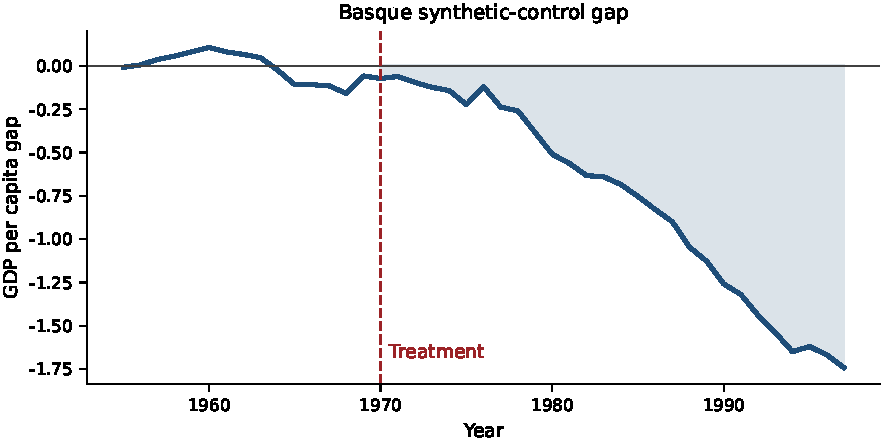
\includegraphics[width=\textwidth]{figures/ex02_basque_gap.pdf}
\caption{Synthetic-control gap (treated minus synthetic per-capita GDP)
for the Basque country under the package-default
\code{sp.synth(method="classic")} path (\(V=I\), outcome-path
predictors) on the calibrated Basque replica, with the
1970 treatment marked. This is the default-convention illustration, not
the ADH parity specification of the parity tables: the parity numbers
come from the special-predictor, nested-\(V\) setup reported in
Section~\ref{sec:scm-identification}. Regenerated by
\code{replication/scripts/generate\_figures.py}; numerical artifacts are
written by \code{replication/scripts/ex02\_basque.py}.}
\label{fig:basque-gap}
\end{figure}

\subsection[Callaway-Sant'Anna staggered DiD: mpdta]{Callaway--Sant'Anna staggered DiD: \texttt{mpdta}}\label{sec:ex-csdid}

The \code{mpdta} example is the main panel-workflow demonstration;
Listing~\ref{lst:csdid} shows the full fit-to-sensitivity chain from one
fitted object.

\begin{lstlisting}[caption={Callaway--Sant'Anna fit, simple- and
event-study aggregation, Rambachan--Roth Honest-DiD bounds, and the
Goodman--Bacon decomposition --- all from the same fitted
object.},label={lst:csdid},captionpos=b]
mpdta = sp.datasets.mpdta()
cs  = sp.callaway_santanna(mpdta, y="lemp", t="year", i="countyreal",
                           g="first_treat", control_group="nevertreated",
                           estimator="reg")
agg = sp.aggte(cs, type="simple", random_state=0)
es  = sp.aggte(cs, type="dynamic", random_state=0)
hd  = sp.honest_did(cs, e=0, method="smoothness")
bd  = sp.bacon_decomposition(mpdta, y="lemp", treat="treat",
                             time="year", id="countyreal")
\end{lstlisting}

\code{sp.callaway\_santanna} estimates group-time ATTs,
\code{sp.aggte} reports simple and dynamic aggregations,
\code{sp.honest\_did} applies the Rambachan--Roth sensitivity
post-estimator, and \code{sp.bacon\_decomposition} gives the TWFE
weight diagnostic \citep{goodmanbacon2021difference}.
Listing~\ref{lst:csdid-output} prints the two objects a reader of this
literature would want to see: the aggregated effect, and how much
parallel-trends violation it survives.

\Needspace*{16\baselineskip}
\begin{lstlisting}[caption={The simple aggregation and the
Rambachan--Roth smoothness bounds from the fit of
Listing~\ref{lst:csdid}. \code{M} is the bound on how much the
post-treatment trend may deviate from the linear extrapolation of the
pre-treatment trend; \code{rejects\_zero} is whether the robust
confidence set still excludes zero at that
bound.},label={lst:csdid-output},captionpos=b]
>>> print(f"{float(agg.estimate):.6f}  {float(agg.se):.6f}")
-0.032977  0.007961
>>> print(hd.round(4).to_string(index=False))
     M  ci_lower  ci_upper  rejects_zero
0.0000   -0.0546   -0.0214          True
0.0037   -0.0566   -0.0129          True
0.0074   -0.0582   -0.0017          True
0.0112   -0.0601    0.0058         False
0.0149   -0.0632    0.0106         False
0.0223   -0.0706    0.0180         False
\end{lstlisting}

The reading is the one \citet{rambachan2023more} intend: the
first-period effect is robust to a post-treatment trend deviation of up
to about \code{M} \(= 0.0074\) log points, and the confidence set
admits zero once the allowed deviation reaches \(0.0112\). That
breakdown value, not the pre-trend test's \(p\)-value, is the quantity
a referee should be given, and it comes off the same fitted object as
the point estimate.

That last clause is the case for the shared contract, and it can be
measured. The Rambachan--Roth interval needs the \emph{joint} covariance
of the event-study coefficients, the relative times, and the position of
the reference period. Composed by hand, the workflow extracts these from
one package's aggregation object and re-enters them into another's
sensitivity function; the tempting shortcut is to rebuild the covariance
from the reported standard errors. On \texttt{mpdta} the pre- and
post-period coefficients are correlated up to 0.61, and the shortcut is
not innocuous: with \(\operatorname{diag}(\mathrm{SE}^2)\) in place of the
joint covariance the breakdown value rises from 0.0080 to 0.0101, so the
estimate would be reported as surviving trend deviations 26\% larger
than the data support, and the \(M=0\) interval shifts from
\([-0.0546,-0.0214]\) to \([-0.0477,-0.0156]\). In \statspai{},
\code{sp.honest\_did} reads the joint covariance, the relative times, and
the aggregation weights from the fitted object through one extractor,
\code{sp.event\_study\_vcov}, shared by nine event-study estimators; when
a fit cannot supply a joint covariance it says so and falls back to a
labelled approximation rather than fabricating one from standard errors.
The single entry point also means a correctness fix applies once: the
1.30.0 repair of the cohort-share term in that covariance
(Table~\ref{tab:correctness-history}) reached every estimator's
sensitivity analysis at the same time. The saving is not lines of code;
it is that the covariance, the reference period, and the estimand
travel with the estimate instead of being re-typed. The \code{random\_state=0} in
Listing~\ref{lst:csdid} is not decoration: \code{sp.aggte} follows
\pkg{did} in defaulting to a 1{,}000-draw multiplier bootstrap, so the
aggregated standard error is a random quantity and a printed
transcript of it is only reproducible once the draw is pinned. The
parity
evidence sits on two data sets, and the paper keeps them apart. On the
calibrated \texttt{mpdta} replica of Track~A module 04,
\statspai{}, \pkg{did}, and \code{csdid} all return the simple ATT
\(-0.0329765\) in the R-joined harness and agree within the registered
iterative tolerance on the analytic SE. On the \emph{original}
\code{did::mpdta} bytes, \statspai{} and \pkg{did} return the simple
ATT \(-0.03995\) at relative error \(2.3\times10^{-14}\) and the
vignette-printed overall dynamic ATT \(-0.0772\) at
\(1.6\times10^{-14}\) (Table~\ref{tab:headline-parity}). The
homogeneous calibrated
replica additionally checks that Callaway--Sant'Anna, Sun--Abraham
\citep{sun2021estimating}, BJS/imputation \citep{borusyak2024revisiting},
and DR-DiD \citep{santanna2020doubly} collapse to the same estimand when
their identification restrictions coincide.
Figure~\ref{fig:mpdta-es} is the printed event-study counterpart to
Listing~\ref{lst:csdid}.

\begin{figure}[!ht]\centering
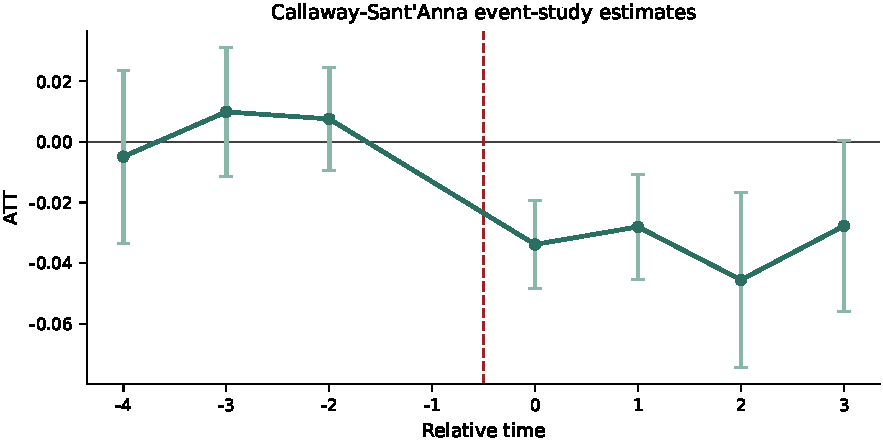
\includegraphics[width=\textwidth]{figures/ex03_mpdta_event_study.pdf}
\caption{Callaway--Sant'Anna dynamic event study on \texttt{mpdta}
(\code{sp.aggte(cs, type="dynamic")}): event-time ATTs with
simultaneous confidence bands. Regenerated by
\code{replication/scripts/generate\_figures.py}; numerical artifacts are
written by \code{replication/scripts/ex03\_csdid.py}.}
\label{fig:mpdta-es}
\end{figure}

\subsection[RD incumbency advantage (Lee-style sharp design)]{Regression discontinuity: the incumbency advantage (Lee-style sharp design)}\label{sec:ex-rd}

The RD example deliberately separates the local-polynomial estimator
from the bandwidth selector, and it keeps two data objects distinct to
avoid over-claiming. The \emph{exact} cross-language parity anchor is
the public \code{rdrobust::RDsenate} extract --- the U.S.\ Senate
margin-of-victory sample distributed with \pkg{rdrobust}, a Lee-style
sharp RD but \emph{not} \citet{lee2008randomized}'s original House
data, which we do not redistribute. The calibrated
\code{lee\_2008\_senate()} replica is a redistribution-safe
drift-guard, not a parity target: on it \code{sp.rdrobust} returns a
robust jump of \(0.0763\), and the external test only asserts that the
estimate stays in the \([0.05,0.12]\) structural neighbourhood.
On the RDsenate extract the native \code{sp.rdrobust} default, which
implements the \citet{calonico2014robust} CCT bandwidth cascade and
robust bias-corrected inference in \statspai{} itself
\citep[software article:][]{calonico2015rdrobust}, returns the same
MSE-optimal bandwidth (17.7544) and conventional and robust estimates as
\proglang{R}'s default \pkg{rdrobust} at relative error below
\(3\times10^{-13}\) (Section~\ref{sec:track-a}). Users who prefer the
authors' own code can call \code{sp.rdrobust(..., bwselect="cct")},
which delegates to the official \pkg{rdrobust} \proglang{Python} port;
the two agree to \(2\times10^{-13}\), and that agreement is recorded as
a convergence check rather than counted as parity. The previous
density-test selector gap is closed by the native \code{sp.rddensity}
port (Section~\ref{sec:track-a}).

\subsection{LaLonde (1986) / Dehejia--Wahba (1999): the NSW programme}\label{sec:ex-lalonde}

The LaLonde \citep{lalonde1986evaluating} / Dehejia--Wahba
\citep{dehejia1999causal} workflow shows the same mature result surface
under an experimental benchmark and an observational comparison. On
\code{causalsens::lalonde.psid} \citep{blackwell2014selection}, the naive OLS ATT is
\(-\$15{,}200\) in both \statspai{} and \proglang{R}, and the
covariate-adjusted OLS ATT is \(\$751.9\) on both sides; on
\code{MatchIt::lalonde}, 1:1 nearest-neighbour PSM agrees with
\pkg{MatchIt} up to the registered caliper/default convention. The
replication script also emits balance and overlap diagnostics: the
point is not that matching fixes the benchmark, but that the platform
keeps the experimental anchor, observational bias, and preprocessing
diagnostics in one auditable pipeline.

\subsection{Causal time series: advertising lift}\label{sec:ex-causal-impact}

The causal-impact example uses a deterministic Brodersen-style
\citep{brodersen2015inferring} advertising-lift simulation rather than
proprietary marketing data.
The known post-intervention lift is \(4.2\) sales units per day;
\code{sp.causal\_impact} estimates \(4.306\) with SE \(0.140\), a 95\%
interval \([4.032,4.579]\), cumulative effect \(129.2\) against true
\(126.0\), and pre-period RMSE \(0.562\). These numbers are not
cross-language parity claims; they are known-truth guards that the
time-series counterfactual machinery, the result object, and the
publication export path are wired correctly.

\subsection{Three ecosystems, one number: panel counterfactuals and interaction effects}\label{sec:ex-fect}

The last example shows the same estimator returning the same number in
all three languages rather than a \proglang{Python} replica of a
published figure. It uses two method families from one research group
that ship their own \proglang{R} and \proglang{Stata} implementations: the counterfactual estimators for
time-series cross-sectional data of \citet{liu2024practical} (\pkg{fect};
two-way fixed effects, interactive fixed effects, and matrix completion,
all fitted on the untreated cells and imputing the treated ones) and the
interaction-effect diagnostics of \citet{hainmueller2019much}
(\pkg{interflex}; the linear, binning, and kernel estimators of a
conditional marginal effect). \statspai{} ports both natively:
\code{sp.fect} runs \pkg{fect}'s EM map step for step, and
\code{sp.interflex} reproduces the \proglang{R} package's conventions
down to the linear-binning-plus-FFT density grid behind its adaptive
kernel bandwidth. Listing~\ref{lst:fect} shows the workflow on the
staggered two-factor panel of parity module 86: a \pkg{panelView}-style
look at the treatment pattern \citep{mou2023panel}, the three
counterfactual fits, and the interaction diagnostics on the module-87
sample.

\begin{lstlisting}[caption={Panel counterfactuals and interaction
effects. \code{sp.panel\_view} reports adoption timing, reversals, and
missing cells before any model is fitted; \code{sp.fect} imputes the
untreated outcome of every treated cell under three outcome models;
\code{sp.interflex} estimates how the treatment effect varies with a
moderator and tests the linear-interaction restriction.},label={lst:fect},captionpos=b]
fig, ax, info = sp.panel_view(panel, unit="id", time="time",
                              treat="D")
info["staggered"], info["has_reversals"]       # (True, False)
fe  = sp.fect(panel, y="Y", treat="D", unit="id", time="time",
              covariates=["X1", "X2"], method="fe")
ife = sp.fect(panel, y="Y", treat="D", unit="id", time="time",
              covariates=["X1", "X2"], method="ife", r=2,
              vce="bootstrap", n_boot=200, seed=0)
mc  = sp.fect(panel, y="Y", treat="D", unit="id", time="time",
              covariates=["X1", "X2"], method="mc", lam=0.002)
ife.detail                              # ATT by relative period
bins = sp.interflex(sample, y="Y", d="D", x="X", z=["Z1"],
                    estimator="binning", cutoffs=[0.3, 1.7])
bins.model_info["tests"]["p_wald"]      # linear vs binning
kern = sp.interflex(sample, y="Y", d="D", x="X", z=["Z1"],
                    estimator="kernel", bw=1.0)
\end{lstlisting}

One scope boundary must be stated before the numbers: the \proglang{R}
\pkg{fect} and \pkg{interflex} packages select the factor number
\(r\), the matrix-completion penalty \(\lambda\), and the kernel
bandwidth by cross-validation by default, and cross-validation draws
random folds. The three-way parity claim below is therefore
established at \emph{user-specified} tuning values (the listing's
\code{r=2}, \code{lam=0.002}, and \code{bw=1.0} are the values fixed
by parity modules 86--87 so that all three implementations solve the
same problem). Since 1.29.0 the selectors themselves are
ported (\code{sp.fect(cv=True)}, \code{sp.interflex(cv=True)}) and
graded T3 rather than T2 by construction: on identical folds the
per-fold scores equal \pkg{fect}'s to \(5.9\times10^{-8}\) and
\pkg{interflex}'s to \(2.8\times10^{-13}\), and across twenty
\proglang{R} fold seeds the selected \(r\), \(\lambda\) and bandwidth
agree with \proglang{R}'s modal choice, with the CV curves inside the
across-seed Monte Carlo spread
(\code{tests/reference\_parity/test\_fect\_interflex\_cv\_parity.py}).
The fit at a CV-selected value equals the fit at that value supplied
by hand, so the T2 rows above are unchanged by the port.

Table~\ref{tab:ex08-three-way} sets the \statspai{} numbers next to
the \proglang{R} and \proglang{Stata} goldens of the parity harness. The
three calls that produce the interactive-fixed-effects row are
\code{sp.fect(..., method="ife", r=2)},
\code{fect(Y ~ D + X1 + X2, method = "ife", r = 2, force = "two-way")},
and \code{fect Y, treat(D) unit(id) time(time) cov(X1 X2) method("ife")
r(2)}; each is given the same CSV bytes, and the ATT agrees to
\(4\times10^{-16}\) with \proglang{R} and \(3\times10^{-10}\) with
\proglang{Stata}. The two rows that are deliberately \emph{not}
three-way are as informative as the rest. The \proglang{Stata}
\code{interflex} command uses a fixed Gaussian kernel where the
\proglang{R} package adapts the bandwidth to the moderator's density,
and it tests the linear restriction without the covariate-by-bin terms
and against an \(F\) reference; \code{sp.interflex} exposes both choices
(\code{adaptive=}, \code{wald\_full\_moderate=}, \code{wald\_test=}) and
reproduces each side to machine precision, so the difference between
the two references is a documented option rather than an unexplained
gap. The complete row set (105 rows for \pkg{fect}, 25 for
\pkg{interflex}, the by-period ATT paths included) is in the parity
ledger.

\begin{table}[!ht]
\centering\scriptsize
\begingroup
\setlength{\tabcolsep}{3pt}
\begin{tabular}{@{}p{0.34\linewidth}rrrrr@{}}
    \toprule
    Quantity & \statspai{} & \proglang{R} & \proglang{Stata} & rel(sp,R) & rel(sp,Stata) \\
    \midrule
    \multicolumn{6}{@{}l}{\emph{fect counterfactual estimators (module 86, staggered two-factor panel)}} \\
    ATT, two-way FE (imputation) & 2.500105 & 2.500105 & 2.500105 & $1.8\times10^{-13}$ & $9.8\times10^{-10}$ \\
    ATT, interactive FE, r = 2 & 2.241884 & 2.241884 & 2.241884 & $4.0\times10^{-16}$ & $2.8\times10^{-10}$ \\
    ATT, matrix completion, lambda = 0.002 & 2.398529 & 2.398529 & 2.398529 & $2.8\times10^{-15}$ & $2.1\times10^{-10}$ \\
    \multicolumn{6}{@{}l}{\emph{interflex marginal effects (module 87, binary treatment, moderator $X$, covariate $Z$)}} \\
    linear ME at the grid midpoint & 3.05408 & 3.05408 & 3.05408 & $5.8\times10^{-16}$ & $2.0\times10^{-15}$ \\
    binning effect, bin 1 (median x = -0.27) & 1.51604 & 1.51604 & 1.51604 & $3.2\times10^{-15}$ & $5.9\times10^{-16}$ \\
    binning effect, bin 2 (median x = 1.06) & 3.18212 & 3.18212 & 3.18212 & $2.8\times10^{-16}$ & $0$ \\
    binning effect, bin 3 (median x = 2.25) & 4.10838 & 4.10838 & 4.10838 & $1.1\times10^{-15}$ & $4.3\times10^{-16}$ \\
    Wald p-value, linear vs binning (R convention) & $7.121\times10^{-7}$ & $7.121\times10^{-7}$ & --- & $6.5\times10^{-13}$ & --- \\
    Wald p-value (Stata convention: no covariate-by-bin terms, F) & $2.249\times10^{-7}$ & --- & $2.249\times10^{-7}$ & --- & $1.2\times10^{-12}$ \\
    kernel ME at the midpoint, adaptive bandwidth (R convention) & 3.34108 & 3.34108 & --- & $2.0\times10^{-15}$ & --- \\
    kernel ME at the midpoint, fixed bandwidth (Stata convention) & 3.27765 & --- & 3.27765 & --- & $1.1\times10^{-15}$ \\
    \bottomrule
\end{tabular}

\endgroup
\caption{Same bytes, three implementations. \statspai{} is re-estimated
by \code{replication/scripts/ex08\_fect\_interflex.py}; the \proglang{R}
(\pkg{fect} 2.4.1, \pkg{interflex} 1.4.0) and \proglang{Stata}
(\code{fect\_stata}, SSC \code{interflex}) columns are the frozen
Track~A goldens of modules 86 and 87. ``---'' marks a quantity the named
reference does not report or computes under a different convention
(shown on its own row).}
\label{tab:ex08-three-way}
\end{table}

\subsection{Cross-example summary}\label{sec:ex-summary}

Together, the examples exercise the same workflow repeatedly:
data-loading, estimator dispatch, typed result objects, diagnostics,
sensitivity/audit calls, citation checks, JSON export, and manuscript
table generation. The examples also enforce the paper's central
boundary: original-data rows are claimed only where the public extract
can be redistributed or regenerated from a reference package, while
deterministic replicas are described as structural guards on sign,
scale, and workflow shape.

\section{Numerical parity and statistical validity}\label{sec:parity}

The empirical claim of this paper is intentionally narrower than the
package surface. \statspai{} registers \RegistryTotal{} public
callables, and the census behind the claim is reported once, here: \RegistryCertified{}
are \code{certified} and \RegistryValidated{} \code{validated}
(together \RegistryCertifiedValidated{}), \RegistryApiStable{} are
\code{api\_stable}, and \RegistryExperimental{} are experimental. The
word ``validated'' in this submission means that a function is in the
\code{certified} or \code{validated} registry tier, and the tiers are
earned in exactly two ways: \code{certified} by a cross-language
comparison with a named reference on identical bytes, \code{validated}
by known-truth recovery or replication of published numbers. Monte
Carlo coverage rows and documented disagreements (T4) are recorded
against a function but never earn a tier on their own, so a disclosure
cannot be read as a demonstration. All \RegistryStableHandwritten{}
hand-written stable symbols carry parity, reference, or API-contract
evidence; the remaining \RegistryAutoUnbacked{} stable auto-registered
symbols are API-stable but not parity-backed, a denominator revisited
in Section~\ref{sec:discussion}. Every \code{certified} symbol is
linked in the registry to a named external reference implementation and
the tolerance it was held to --- an \proglang{R} or \proglang{Stata}
parity module for all but a handful whose canonical implementation is a
\proglang{Python} package (\pkg{econml}, \pkg{DoubleML}, \pkg{pyblp},
\pkg{obp}); those exceptions are enumerated in the package
(\code{PYTHON\_REFERENCE\_ROWS}) and asserted by a test.
Every \code{validated} symbol is linked to at least one known-truth or
published-replication artifact; the validation-evidence audit in the archive fails on any
certified/validated symbol whose registry entry lacks such an
attachment, so the mapping from the \RParityModuleCount{} modules to
the \RegistryCertifiedValidated{} certified/validated symbols is
enumerable rather than asserted.

Two properties of that census are easy to misread, so both are stated
here rather than left to be recomputed. First, the certified and
validated tiers answer different questions and are not summed in this
paper's coverage language. \ParityCrossLanguage{} symbols were compared
against a named \proglang{R} or \proglang{Stata} implementation on
identical inputs; \ParityInternalEvidence{} recover a known population
parameter on a deterministic DGP or reproduce published numbers on a
calibrated replica. Only the first is a parity claim. The second is the
strongest evidence available for a method with no reference
implementation, and reporting a combined figure would let it borrow the
first one's authority. Second, the all-registered denominator dilutes
coverage: of \RegistryTotal{} registered callables, \ParityClassTotal{}
are result or exception classes that can never carry a parity grade and
\ParityInfraTotal{} are infrastructure that renders tables, draws plots,
builds agent schemas or loads data. Against the \ParityEstimatorTotal{}
estimator callables that remain, cross-language coverage is
\ParityEstimatorCrossLanguage{} functions
(\ParityEstimatorCrossLanguagePct{}). \code{sp.parity\_summary()} returns
this split at call time, so a reader never has to reconstruct the
denominator from a printed total.

The registry tier and the parity grade are derived from one artifact,
the committed parity index, through a single grade-to-tier function; a
test asserts that the two agree for every stable symbol.

The validation design is a twelve-estimator suite with four evidence
tracks: numerical parity (Track A), Monte Carlo coverage against known
DGPs (Track B, separated into materialized \(B_{1000}\) rows and
estimator-specific slow-suite \(B_s\) rows), computational scaling (Track C,
Section~\ref{sec:performance}), and agent-facing mechanical checks
(Track D, Section~\ref{sec:agentbench}).
This is representative, not exhaustive: it covers the causal-inference
core behind the paper's statistical evidence claims, not every
auxiliary helper in the registry.

Because the paper uses several graded vocabularies, Table~\ref{tab:terminology}
fixes them before any evidence is read. The practical
reading rule is as follows. A \code{certified} or
\code{validated} label is local to the named function, data contract,
and evidence kind recorded in the registry; it does not promote nearby
helpers or optional backends, and only a T2 row is a parity claim.
Conversely,
\code{api\_stable} means that the call signature and output shape are
stable enough to support user code, not that the estimator has the
paper-level statistical evidence required for a validation claim.

\begin{table}[tbp]
\centering\small
\begin{tabular}{p{0.24\linewidth}p{0.70\linewidth}}
\toprule
Vocabulary & Meaning \\
\midrule
Registry tiers & \code{certified} / \code{validated} / \code{api\_stable} /
\code{experimental}: the per-function evidence label queryable at call
time (Section~\ref{sec:registry}). \\
Evidence grades T1--T5 & Kind of numerical evidence behind a row:
known-truth recovery (T1), same-byte cross-language parity (T2),
seed-replicated equivalence of a stochastic estimator within a stated
margin (T3), documented
convention or identification boundary (T4), registered but not
validated here (T5) (Section~\ref{sec:validation-tiers}). \\
Tracks A--D & The four evidence tracks of the validation suite: parity,
coverage, performance, agent-facing mechanical checks. \\
\(B_{1000}\), \(B_s\) & Monte Carlo draw counts: materialized
1{,}000-draw rows versus the slower estimator-specific suite. \\
Reviewer paths & The three reproduction routes of
Section~\ref{sec:reproducibility}: the licence-free \proglang{Python}
path, the pinned-\proglang{R} path, and the \proglang{Stata} path. \\
\bottomrule
\end{tabular}
\caption{Terminology used by the validation sections. Each vocabulary is
orthogonal: a \code{certified} function can carry T2 and T4 rows on
different fixtures, and any row can be rebuilt on one or more reviewer
paths.}
\label{tab:terminology}
\end{table}

\subsection{Twelve-estimator validation suite}\label{sec:decathlon}

\begin{table}[!ht]
\centering\small
\begingroup
\setlength{\tabcolsep}{3pt}
\begin{tabular}{@{}rL{0.17\linewidth}L{0.26\linewidth}L{0.24\linewidth}L{0.15\linewidth}l@{}}
\toprule
\# & Method & Entry point & Reference & Data / DGP & Tracks \\
\midrule
1  & OLS + HC SE             & \code{sp.regress}         & \code{lm}+\pkg{sandwich}; \code{regress} & Card 1995 & A,\(B\),D \\
2  & 2SLS                    & \code{sp.iv}              & \pkg{AER}; \code{ivregress} & Card 1995 & A,\(B\),D \\
3  & HDFE                    & \code{sp.fast.feols}      & \pkg{fixest}; \code{reghdfe} & HDFE panel & A,\(B\),C,D \\
4  & Callaway--Sant'Anna     & \code{sp.callaway\_santanna} & \pkg{did}; \code{csdid} & \texttt{mpdta} & A,\(B\),C,D \\
5  & Sun--Abraham            & \code{sp.sun\_abraham}    & \pkg{fixest}; \code{eventstudyinteract} & \texttt{mpdta} & A,\(B\),D \\
6  & Bias-corrected RD       & \code{sp.rdrobust}        & \pkg{rdrobust}; \code{rdrobust} & RDsenate & A,\(B\),D \\
7  & RD density test         & \code{sp.rddensity}       & \pkg{rddensity}; \code{rddensity} & RDsenate & A,D \\
8  & Classical SCM           & \code{sp.synth}           & \pkg{Synth}; \code{synth} & Basque; unique DGP & A,C,D \\
9  & Synthetic DID           & \code{sp.sdid}            & \pkg{synthdid}; \code{sdid} & California-99 & A,\(B\),D \\
10 & DML PLR                 & \code{sp.dml}             & \pkg{DoubleML} & Card/401(k) & A,\(B\),C,D \\
11 & Causal forest           & \code{sp.causal\_forest}  & \pkg{grf} & Clean-overlap DGP & A,\(B\),D \\
12 & PSM                     & \code{sp.psm}             & \pkg{MatchIt}; \code{teffects} & NSW-DW & A,D \\
\bottomrule
\end{tabular}
\endgroup
\caption{Twelve-estimator validation suite. In the Reference column the
\proglang{R} package precedes the \proglang{Stata} command. Tracks are A
(parity), \(B\) (materialized 1,000-draw coverage), C (performance), and
D (agent-facing mechanical checks); row 8 dispatches as
\code{sp.synth(method="classic")} and row 10 as
\code{sp.dml(model="plr")}. Data marked with a named extract are
calibrated replicas in Track~A and original extracts in
Table~\ref{tab:headline-parity}. The HDFE member's coverage row
runs through the \code{sp.panel} fixed-effects entry of the same
absorption family. Supplemental Track-B rows for
2x2 DiD and entropy balancing are reported in
Table~\ref{tab:track-b-b1000} but are not members of this suite.}
\label{tab:decathlon}
\end{table}

The reference implementations of Table~\ref{tab:decathlon} are cited
once here: \code{lm} with \pkg{sandwich} \citep{zeileis2020sandwich},
\pkg{AER}'s \code{ivreg} \citep{kleiber2008applied}, \pkg{fixest}
\citep{berge2018efficient}, \pkg{did} \citep{callaway2021difference},
\pkg{rdrobust} \citep{calonico2014robust,calonico2015rdrobust},
\pkg{rddensity} \citep{cattaneo2018manipulation,cattaneo2020simple},
\pkg{Synth} \citep{abadie2011synth}, \pkg{synthdid}
\citep{arkhangelsky2021synthetic}, \pkg{DoubleML}
\citep{bach2022doubleml,bach2024doubleml}, \pkg{grf}
\citep{athey2019generalized}, and \pkg{MatchIt} \citep{ho2011matchit},
with the \proglang{Stata} commands \code{csdid} \citep{rios2022csdid},
\code{sdid} \citep{clarke2024synthetic}, \code{eventstudyinteract}
\citep{sun2021estimating}, and \code{reghdfe}'s Poisson companion
\code{ppmlhdfe} \citep{correia2020fast}.

\subsection{Estimands, identification, and inference contracts}
\label{sec:statistical-contracts}

Numerical agreement does not establish identification. This subsection
therefore states the contract under which each validation-suite row has a
causal interpretation. These are
contracts on the user's design and data, not properties that software can
certify from a successful function call.  In particular, parity with a
reference implementation can establish that two programs compute the same
quantity while both remain inappropriate for a design that violates
exogeneity, parallel trends, continuity, or overlap.

For the linear rows, write \(Y=X\beta+u\).  The OLS coefficient is always a
linear-projection parameter; interpreting it causally additionally requires
the relevant conditional-mean restriction.  With instruments \(Z\), 2SLS
solves the sample analogue of \(E[Z(Y-X\beta)]=0\); a LATE interpretation for
a binary treatment further requires relevance, independence, exclusion, and
monotonicity.  Absorbing fixed effects changes the projection space, not these
identification requirements.  The parity harness specifies the covariance
estimator explicitly---HC1 or the named cluster---rather than relying on the
entry point's non-robust default.

For staggered adoption, the target primitive is

\[
  \operatorname{ATT}(g,t)
  = E\!\left[Y_t(1)-Y_t(0)\mid G=g\right],
\]

identified under no anticipation, a stated never-treated or not-yet-treated
comparison group, conditional parallel trends, overlap, and no interference.
Callaway--Sant'Anna aggregates these group--time effects; Sun--Abraham first
forms cohort-by-relative-time effects and then interaction weights.  A joint
pre-trend test is reported, but failure to reject is not proof of parallel
trends and its power must be considered.

The RD row targets the sharp/fuzzy cutoff effect (or kink contrast) under
continuity, local support, and no precise manipulation; its parity row
uses the native robust bias-corrected interval at the native CCT
MSE-optimal bandwidth (Section~\ref{sec:track-a}).

The remaining rows target nonparametric discontinuities, counterfactual
panels, or effects learned after nuisance estimation.  For RD density the null
is equality of the one-sided density limits at the cutoff; rejecting it is a
design diagnostic, not itself an effect estimate.  Classical SCM and SDID
construct weighted untreated counterfactuals, so pre-treatment fit and the
stability of the untreated outcome process are central.  Their placebo
distributions are design-based diagnostics and should not be read as generic
i.i.d. sampling distributions. SDID uses placebo inference by default
(with bootstrap and jackknife alternatives), while classical SCM offers
in-space placebos.

DML PLR uses an orthogonal, cross-fitted score for the partially linear model
\(Y=\theta D+g(X)+\varepsilon\), \(D=m(X)+v\).  A causal reading of
\(\theta\) requires the corresponding conditional exogeneity and overlap
conditions in addition to nuisance-rate conditions.  The forest row targets
\(\tau(x)=E[Y(1)-Y(0)\mid X=x]\); its ATE/ATT summaries use an AIPW score and
therefore require conditional exchangeability and overlap.  PSM targets ATT
by default and requires conditional exchangeability, common support, and a
credible propensity specification.  Balance and overlap diagnostics remain
part of the analysis even when the reference parity row passes. The validation
path uses five-fold DML cross-fitting, AIPW influence-function intervals for
forest aggregates, and Abadie--Imbens heteroskedastic inference for default
nearest-neighbour PSM.

\subsection{Track A: Numerical parity}\label{sec:track-a}

Track A uses three layers. First, estimators are tested against known
DGP truths whenever a truth exists. Second, \statspai{} and the
canonical \proglang{R} implementation read the same \code{\%.16g} CSV
bytes and write full-precision JSON. Third, when a directly comparable
\proglang{Stata} command exists, the Stata side reads the same CSV and
emits a sibling JSON artifact. The current R-joined harness has
\RParityModuleCount{} modules. Of those, \StataParityModuleCount{} carry a
canonical or audited Stata reference; each of the
\NoStataModuleCount{} without one records a measured, command-level
reason in \code{compare.py::STATA\_SKIP\_REASON}.
Rows whose defaults differ for a documented reason are labelled as
convention gaps rather than as ordinary passes.
Table~\ref{tab:internal-parity} summarizes the source-tree test layers
behind these claims.

\begin{table}[!ht]
\centering\small
\begin{tabular}{p{0.25\linewidth}p{0.22\linewidth}rp{0.36\linewidth}}
\toprule
Layer & Harness & Tests & Role \\
\midrule
Analytical/reference recovery & reference parity & 4{,}285 & Deterministic-DGP recovery, frozen \proglang{R} / \proglang{Stata} reference fixtures on identical bytes, and cross-estimator agreement; includes the 203 tests that pin Stata's \code{vce()} grammar (27 estimators, 79 estimator-by-covariance cells at \(10^{-6}\)) and its \code{test}, \code{lincom} and \code{margins} post-estimation commands \\
Published/replica parity & external parity & 88 & Pinned values for Card, Lee, Basque, NSW, \texttt{mpdta}, paper-level formulas, and the four \pkg{DoubleML} model-class pins \\
Monte Carlo coverage & coverage MC & 32 & Slow-marked headline DGP checks, robustness rows, and one smoke row \\
\bottomrule
\end{tabular}
\caption{Validation test layers available in the source tree used for
this submission. Counts are the tests \code{pytest} collects in each
harness, reported by \code{sp.validation\_report(collect\_tests=True)}
and pinned as floors by \code{tests/test\_jss\_validation\_api.py}; the
Track A modules of Appendix~\ref{app:parity} are a separate,
module-level artifact.}
\label{tab:internal-parity}
\end{table}

\begin{table}[!ht]
\centering\scriptsize
% AUTO-GENERATED by tests/r_parity/compare.py
% Compact main-manuscript Track A snapshot; do not hand edit.
\setlength{\tabcolsep}{2pt}
\begin{tabular}{@{}>{\raggedright\arraybackslash}p{0.195\linewidth}>{\raggedright\arraybackslash}p{0.106\linewidth}>{\raggedright\arraybackslash}p{0.084\linewidth}r@{\hspace{3pt}}r@{\hspace{3pt}}r@{\hspace{4pt}}r@{\hspace{4pt}}>{\raggedright\arraybackslash}p{0.115\linewidth}@{}}
\toprule
Estimator & Statistic & Data & \statspai{} & \proglang{R} ref. & \proglang{Stata} ref. & Max rel. err. & Verdict \\
\midrule
\code{sp.fast.feols} & \(\hat\beta_{x1}\) & 2-way HDFE, \(N{=}10^4\) & 1.999503980 & 1.999503980 & 1.999503980 & \(2.9\times10^{-15}\) & T2; fixest ssc \\
\code{sp.regress} & \(\hat\beta_{\mathrm{educ}}\) & Card replica & 0.109986249 & 0.109986249 & 0.109986249 & \(6.3\times10^{-13}\) & T2 \\
\code{sp.iv} & \(\hat\beta_{\mathrm{educ}}\) & Card replica & 0.141834409 & 0.141834409 & 0.141834409 & \(1.1\times10^{-11}\) & T2 \\
\code{sp.callaway\_santanna} & simple ATT & \texttt{mpdta} replica & -0.032976514 & -0.032976514 & -0.032976514 & \(1.3\times10^{-15}\) & T2 \\
\code{sp.rdrobust} & robust RD, default CCT \(h\) & RDsenate & 7.506502484 & 7.506502484 & 7.506502483 & \(9.4\times10^{-11}\) & T2; native, default \(h\) \\
\code{sp.dml} & \(\hat\theta_{\mathrm{DML}}\) & Card replica & 0.110228260 & 0.110228260 & 0.110228260 & \(3.7\times10^{-15}\) & T2; ddml bridge \\
\code{sp.causal\_forest} & AIPW ATE & clean-overlap DGP & 1.012009376 & 1.011741552 & --- & 0.000265 & T3; seed-replicated, operator exact \\
\code{sp.psm} & ATT & NSW--DW replica & 2277.690721 & 2277.690721 & 2277.690721 & \(1.2\times10^{-15}\) & T2; SE convention \\
\code{sp.synth} (unique) & avg post gap & identified SCM DGP & 2.000000155 & 1.999999999 & 2.000000000 & \(7.8\times10^{-8}\) & T1+T2; identified DGP \\
\code{sp.synth} (classic) & avg post gap & Basque replica & -0.704244148 & -0.687789210 & -0.703950536 & 0.0239 & T4; reference disagreement \\
\code{sp.frontier} & intercept & frontier DGP & 2.071558153 & 2.071558166 & 2.071558168 & \(7.2\times10^{-9}\) & T2 \\
\code{sp.decompose} & Oaxaca gap & Oaxaca DGP & 0.221231026 & 0.221231026 & 0.221231026 & \(6.3\times10^{-16}\) & T2 \\
\bottomrule
\end{tabular}

\caption{Representative Track A cross-language parity rows compiled
from the same JSON artifacts as the supplementary parity ledger. Every
row is inside its registered module-level tolerance in
\code{tests/r\_parity/compare.py}, which is \(10^{-6}\) except where
the verdict says otherwise: the DML row's tighter \(10^{-10}\) budget
reflects its fully deterministic linear-learner pipeline, the forest
row is a single draw from each engine whose interpretation rests on the
seed-replicated comparison of Section~\ref{sec:validation-tiers}, and
the classical-SCM row is the \(5\times10^{-2}\) T4 disclosure. Data
marked ``replica'' are the calibrated redistribution-safe fixtures; the
Card-replica rows use the specification \code{lwage \~{} educ + exper +
expersq + black + south + smsa} with HC1 errors, which is why their
coefficients differ from the shorter original-extract specification of
Table~\ref{tab:headline-parity}.}
\label{tab:track-a-cross-language-snapshot}
\end{table}

Table~\ref{tab:track-a-cross-language-snapshot} is only a compact slice;
the full row-level ledger is generated in the replication archive. Its
fixtures are calibrated, redistribution-safe replicas (the Data column
names them as such); original public extracts are handled separately in
Table~\ref{tab:headline-parity}. Of
the \RParityModuleCount{} R-joined modules, \RParityPassCount{} receive a pass-type verdict, but two
non-T2 Track A rows remain explicitly visible in the parity artifacts:
classical SCM on the calibrated Basque replica is a T4
identification/reference-disagreement disclosure,
and causal forest is a stochastic T3 equivalence claim rather than a
deterministic T2 claim.
A parity row is evidence about a \statspai{} algorithm only if the
\proglang{Python} side ran one, so every module is also classified by
what its \statspai{} side executes, and the classification is not taken
on trust: a call-trace audit
(\code{scripts/trace\_parity\_provenance.py}) runs each module under a
profiler that records every call from \statspai{} into a package other
than the numerical substrate (\pkg{NumPy}, \pkg{SciPy}, \pkg{pandas})
and every subprocess it launches, and a contract test fails if the
registered classification and the trace disagree or if a module has
changed since it was traced. Of the \RParityModuleCount{} modules,
\ParityNativeModuleCount{} run a \statspai{}-native implementation
(\pkg{scikit-learn} appears only as a user-chosen nuisance learner);
\ParityThirdPartyModuleCount{} are served by a third-party
\proglang{Python} estimation library that \statspai{} wraps --- panel
fixed and random effects through \pkg{linearmodels}, ARIMA through
\pkg{statsmodels}, and fixed-effects GLMs through \pkg{pyfixest} ---
and are marked as such in Appendix~\ref{app:parity}, because they
validate the wrapper's argument mapping and conventions rather than an
independent algorithm; \ParityPortModuleCount{} rely on an official
port; and \ParityBackendModuleCount{} call a reference implementation.
That last count was two before release 1.31: until then the
two Honest-DiD modules called \code{backend="honestdid"}, which hands the
computation to the \proglang{R} package itself, so their rows compared
\proglang{R} with \proglang{R}; the RD headline delegated to the
official \pkg{rdrobust} \proglang{Python} port. All three now exercise
native code, and each carries evidence of its own. The native
smoothness FLCI is compared with \pkg{HonestDiD} after the package's
simulated folded-normal quantile is replaced by the exact one (the
shipped package sits \(3\times10^{-4}\) away, which is that simulation
error): the bounds agree to \(1.4\times10^{-8}\) for \(M>0\), and at
\(M=0\), where the interval has a closed form (the GLS linear
extrapolation of the pre-period coefficients), the native solver is
within \(2\times10^{-9}\) of it while \pkg{HonestDiD}'s cone solver is
\(5.7\times10^{-6}\) away. The native relative-magnitudes set is a port
of the Andrews--Roth--Pakes conditional test \citep{andrews2023inference}
inverted over \pkg{HonestDiD}'s \(\theta\) grid; on sixteen cases
(diagonal and correlated covariances, a non-basis target, a single
post-period) it returns the \emph{same} accepted grid points as
\pkg{HonestDiD}, and the least-favourable hybrid, whose first-stage
critical value is simulated, agrees to within one grid step. The native
RD default selector returns \pkg{rdrobust}'s MSE-optimal bandwidth and
robust estimate on the RDsenate bytes at relative error below
\(3\times10^{-13}\), with the port recorded only as a convergence check.
Module 52
separately certifies the native classical-SCM solver on a uniquely
identified DGP. A generated ledger in the replication archive
classifies the remaining T4 row and fails the audit if a methodological
gap appears without an explicit reviewer-risk label and promotion path;
the causal-forest row is governed by the seed-replicated comparison of
Section~\ref{sec:validation-tiers}.

Native \code{sp.sdid} matches \pkg{synthdid}'s ATT at relative error
\(2.6\times10^{-15}\) and native \code{sp.rddensity} matches
\pkg{rddensity}'s p-value at \(3.3\times10^{-11}\) \citep{arkhangelsky2021synthetic,cattaneo2020simple}.

\paragraph{Headline original-data rows.}
The Track~A fixtures above are calibrated, redistribution-safe
replicas; the complementary original-data ledger runs \statspai{} and
the canonical \proglang{R} reference on the \emph{original} public
extracts shipped by \proglang{R} packages. It currently holds
\OrigParityModuleCount{} modules and \OrigParityRowCount{} statistic
rows, including six epidemiology-side modules that reproduce the
NHEFS worked examples of Hern\'an and Robins' \emph{What If} (IPW,
g-formula, g-estimation, outcome regression, survival, and E-values).
Table~\ref{tab:headline-parity} shows the most reviewer-relevant
cases; the full report is generated by
\code{tests/orig\_parity/compare\_orig.py}, and the printed table is
itself generated from those artifacts. The \code{did::mpdta}
simple-ATT row makes the replica/original boundary concrete: the
calibrated replica used by Track~A module 04 returns \(-0.0330\) on all
three sides, while the original bytes return \(-0.03995\); both are
same-byte parity facts, and neither number is quoted against the other
data set anywhere in this paper.

\begin{table}[!ht]
\centering\scriptsize
\resizebox{\textwidth}{!}{%
% AUTO-GENERATED by replication/scripts/generate_headline_parity_table.py
% Cells come from tests/orig_parity/results/*.json; do not hand edit.
\begin{tabular}{@{}L{0.24\linewidth}L{0.19\linewidth}rrrL{0.23\linewidth}@{}}
\toprule
Extract & Statistic & Published & \statspai{} & \proglang{R} & Note \\
\midrule
\code{wooldridge::card} & OLS educ & $0.075$ & $0.07401$ & $0.07401$ & rel(sp,R) \(7.9\times10^{-15}\) \\
\code{wooldridge::card} & 2SLS educ & $0.132$ & $0.1323$ & $0.1323$ & rel(sp,R) \(1.6\times10^{-11}\) \\
\code{did::mpdta} & CS simple ATT & -- & $-0.03995$ & $-0.03995$ & rel(sp,R) \(2.3\times10^{-14}\); no printed vignette anchor \\
\code{did::mpdta} & CS dynamic overall ATT & $-0.0772$ & $-0.07724$ & $-0.07724$ & rel(sp,R) \(1.6\times10^{-14}\); vignette prints $-0.0772$ \\
\code{Synth::basque} & ADH avg gap & $-0.855$ & $-0.8946$ & $-0.8944$ & rel(sp,R) \(1.8\times10^{-4}\); Stata \code{synth} $-0.8943$ on the same bytes \\
\code{rdrobust::RDsenate} & robust RD jump & -- & $7.507$ & $7.507$ & rel(sp,R) \(3.5\times10^{-16}\); \code{bwselect="cct"} path \\
\code{causalsens::lalonde.psid} & adjusted OLS ATT & $700$ & $751.9$ & $751.9$ & rel(sp,R) \(2.2\times10^{-13}\); public composite extract \\
NHEFS (\emph{What If}) & IP-weighted ATE & $3.4$ & $3.441$ & $3.441$ & rel(sp,R) \(1.3\times10^{-11}\) \\
NHEFS (\emph{What If}) & g-formula ATE & $3.5$ & $3.463$ & $3.463$ & rel(sp,R) \(7.4\times10^{-12}\) \\
\bottomrule
\end{tabular}
}
\caption{Selected original-data parity rows on public extracts,
generated from \code{tests/orig\_parity/results/}. All \proglang{R}
references read the same CSV bytes as \statspai{}. The \emph{Published}
column is a heterogeneous anchor --- an original-paper table value
(Card, Basque), a printed-vignette value (the \code{did} dynamic ATT),
a textbook program output (NHEFS), or a rounded composite-extract value
(LaLonde) --- shown for context, not as a parity target; the parity
claim is the \statspai{}-versus-\proglang{R} pair in the \emph{Note}
column. The \code{did::mpdta} simple-ATT row has no printed vignette
anchor, so its Published cell is empty by design.}
\label{tab:headline-parity}
\end{table}

\subsection{Evidence tiers and hard cases}\label{sec:validation-tiers}

\paragraph{Evidence is attached to configurations.}
A tier is attached to a function, but every artifact exercises one
configuration: a method variant, an inference option, a data condition,
a code path, and an output. The Track~B DML row is the plain example:
the suite member is the partially linear model, and until this revision
the only materialised coverage row ran the interactive model, which says
nothing about the other's intervals (a PLR row is now included,
Table~\ref{tab:track-b-b1000}). For the twelve suite estimators the
package therefore records, per artifact, the configuration it exercises,
and \code{sp.validation\_scope(result)} reads the configuration of a
fitted object and returns the artifacts that match it exactly
(``covered'' requires a T1 or T2 row; ``stochastic only'' means only
T3, T4, or coverage rows match; otherwise ``not covered''), together
with the artifacts that differ in one dimension. The map is deliberately
narrower than the registry --- an option it does not list is reported as
not covered --- and it found a gap in this paper's own first example:
\code{sp.iv}'s default classical 2SLS covariance, printed in
Listing~\ref{lst:card-output}, had no deterministic reference row
(Track~A pins the HC1 variant). It is now pinned against
\pkg{AER}\code{::ivreg} on the original Card extract, with classical,
HC1, and clustered errors in just- and over-identified models, at
\(8\times10^{-11}\).

\paragraph{Evidence grades.}
The grades are those of Table~\ref{tab:terminology}; T5 marks a function
registered but not validated in this paper. Two rows need more than a
tolerance to read correctly.

\paragraph{Causal forest: which Monte Carlo error?}
For a stochastic estimator two uncertainties must be kept apart:
sampling variation across datasets, which the reported standard error of
the ATE estimates, and the algorithm's own Monte Carlo variation across
seeds on \emph{fixed} data. ``Agreement within combined Monte Carlo
error'' is a statement about the second, so it cannot be tested by
dividing the gap between one \statspai{} fit and one \pkg{grf} fit by
their sampling standard errors --- which is how an earlier version of
this row was graded. The forest evidence now separates three tasks.
\emph{Truth recovery and inference} are Track~B's (the AIPW coverage row
below). \emph{Estimand agreement} holds by construction: both engines
report the doubly-robust AIPW average \citep{athey2019generalized}, and
given the same forest the AIPW operator agrees with \pkg{grf}'s to
machine precision. \emph{Algorithmic agreement} is tested by refitting
each engine under 50 seeds (20 at 8{,}000 trees) on fixed data, at
500, 2{,}000, and 8{,}000 trees, on two datasets: the reference-parity
fixture and the Track~A module-13 design, the latter run after the
equivalence margin was fixed. Seeds are spaced \(10^5\) apart on both
sides, because \pkg{grf} forests grown from consecutive seeds share most
of their random draws: a first run with consecutive \proglang{R} seeds
understated \pkg{grf}'s seed-to-seed spread several-fold and made
\statspai{}'s forest look several times noisier than it is.
Table~\ref{tab:forest-seed-mc} reports the result. At every tree count
on both datasets a two-one-sided test establishes equivalence within
\(\delta = 0.1\) sampling standard errors --- a difference that moves a
95\% interval endpoint by at most 5\% of its half-width --- with an
upper bound of at most 0.056. The two engines are equally noisy: their
seed-to-seed standard deviations differ by a factor between 0.78 and
1.48 and fall with the number of trees, from 13--18\% of the sampling
standard error at 500 trees to 6--8\% at the default 2{,}000. The claim
is equivalence, not identity: the engines are independent
implementations, and at 8{,}000 trees, where Monte Carlo error is
smallest, their seed means differ by up to 0.025 sampling standard
errors (\(|z| \le 2.6\)). The single-fit Track~A row is one draw from
each distribution, not a parity fact on its own.
Artifacts: \path{tests/reference_parity/test_grf_seed_mc_equivalence.py}
and its fixtures.

\begin{table}[!ht]
\centering\footnotesize
% AUTO-GENERATED by replication/scripts/generate_forest_seed_table.py
\begingroup\setlength{\tabcolsep}{3pt}
\begin{tabular}{@{}lrrrrrrrl@{}}
\toprule
Data & Trees & Seeds & Gap & MC SE & Gap/SE\(_s\) & SD\(_{\mathrm{MC}}\) (\statspai{}) & SD\(_{\mathrm{MC}}\) (\pkg{grf}) & Equiv. \\
\midrule
Reference fixture & 500 & 50/50 & -0.00028 & \(2.0\times10^{-3}\) & -0.004 & \(1.0\times10^{-2}\) & \(1.0\times10^{-2}\) & yes \\
 & 2000 & 50/50 & +0.00135 & \(9.2\times10^{-4}\) & +0.018 & \(4.4\times10^{-3}\) & \(4.9\times10^{-3}\) & yes \\
 & 8000 & 20/20 & +0.00139 & \(6.2\times10^{-4}\) & +0.019 & \(2.3\times10^{-3}\) & \(1.5\times10^{-3}\) & yes \\
Module-13 design & 500 & 50/50 & +0.00003 & \(9.8\times10^{-4}\) & +0.001 & \(4.7\times10^{-3}\) & \(5.1\times10^{-3}\) & yes \\
 & 2000 & 50/50 & +0.00015 & \(4.6\times10^{-4}\) & +0.004 & \(2.2\times10^{-3}\) & \(2.4\times10^{-3}\) & yes \\
 & 8000 & 20/20 & -0.00003 & \(3.7\times10^{-4}\) & -0.001 & \(1.0\times10^{-3}\) & \(1.3\times10^{-3}\) & yes \\
\bottomrule
\end{tabular}
\endgroup

\caption{Seed-replicated comparison of \code{sp.causal\_forest} and
\pkg{grf}~2.6.1 on fixed data (AIPW ATE; ATT in the archive).
``Gap'' is the difference of seed means; ``MC SE'' its combined
algorithmic Monte Carlo standard error; ``Gap/SE\(_s\)'' the gap in units
of \pkg{grf}'s reported sampling standard error; ``MC SD'' the seed-to-seed
standard deviation of each engine. Equivalence (TOST, 5\%) against
\(\delta = 0.1\,\mathrm{SE}_s\) holds in every row. Generated by
\code{replication/scripts/generate\_forest\_seed\_table.py}.}
\label{tab:forest-seed-mc}
\end{table}

\paragraph{Synthetic control: one specification, two data sets.}\label{sec:scm-identification}
The classical-SCM row is a T4 disclosure because the outer \(V\)
optimization is non-convex and donor weights need not be unique --- and
how much that matters turns out to be data-dependent, which the ledger
reports rather than averages away. On the \emph{calibrated Basque
replica} of Track~A module 07 (the same ADH special-predictor
specification and CSV bytes on all three sides), native \statspai{}
tracks Stata \code{synth} for the average post-treatment gap at
relative error \(4.2\times10^{-4}\), while R \pkg{Synth} and Stata
\code{synth} differ from each other by \(2.3\times10^{-2}\). On the
\emph{original} \code{Synth::basque} bytes under the same
specification, the three implementations essentially reconvene:
\statspai{} \(-0.8946\), \proglang{R} \(-0.8944\), \proglang{Stata}
\(-0.8943\), pairwise within \(4\times10^{-4}\)
(Table~\ref{tab:headline-parity}) --- still above the \(10^{-6}\)
strict-parity gate, consistent with solver tolerance on a non-convex
outer problem, but far from the replica's split. The same specification
therefore admits a near-common optimum on one data set and measurably
different local optima on another; a validation ledger that pooled the
two facts into one tolerance would hide exactly the sensitivity a
practitioner needs to know about. The solver is
separately certified on an identified SCM DGP (Track~A module 52): when
the treated unit is exactly a unique convex combination of donors,
\statspai{}, \pkg{Synth}, and Stata \code{synth} agree on the average
post-treatment gap at relative error \(7.8\times10^{-8}\) and on the
donor weights at \(5.6\times10^{-7}\), the tolerance of the constrained
quadratic solver. Thus the
paper claims solver correctness on identified problems and documents
the replica's reference-disagreement/local-optimum problem without
treating it as a strict R/Synth parity pass.

Native \code{sp.augsynth} now ports \pkg{augsynth}'s Ridge+SCM
convention \citep{benmichael2021augmented} (ATT at \(7.9\times10^{-6}\)
on the Basque fixture).
Native \code{sp.gsynth} now ports \pkg{gsynth}'s two-way factor
convention \citep{xu2017generalized}, matching it to machine precision.

\subsection{Track B: Monte Carlo coverage}\label{sec:track-b}

Track B checks 95\% interval coverage on known DGPs, and reports with
each rate what is needed to explain it: the estimator's bias, its Monte
Carlo SD, the mean reported standard error, their ratio, and the
interval length (Table~\ref{tab:track-b-b1000}). The artifact holds
twelve \(B=1{,}000\) rows; ten correspond to suite members (OLS, 2SLS,
fixed effects through \code{sp.panel}, Callaway--Sant'Anna,
Sun--Abraham, sharp RD, SDID, DML PLR, and the causal forest), and 2x2
DiD, entropy balancing, and the interactive DML model are supplemental.
Three suite members have no coverage row by construction: the RD density
test is a diagnostic, classical SCM has no analytic interval, and PSM's
inference evidence is the Abadie--Imbens SE parity row.

Most rows are calibrated in the direct sense: the mean standard error is
within 3\% of the Monte Carlo SD and coverage sits in the 99\% Wilson
band around 0.95. The rows that are not are explained rather than
graded. \emph{Sharp RD} (0.934) and \emph{SDID} (0.928) have calibrated
standard errors (ratios 0.98 and 0.99), so the shortfall is in the shape
of the sampling distribution, not the SE. For RD this is the reference
procedure's own finite-sample behaviour: on the first 200 draws R
\pkg{rdrobust}~4.0.0 returns the same intervals as \statspai{} to
\(6\times10^{-12}\) and covers in exactly the same draws
(\path{tests/coverage_monte_carlo/mechanisms/rd_drawwise_reference.py}).
\emph{DML PLR} under-covers clearly (0.883), and the diagnostics say why:
its bias is half a Monte Carlo SD while the SE is nearly calibrated
(0.88). \code{sp.dml} returns \pkg{DoubleML}'s numbers to \(10^{-16}\) on
the same folds and learners, so this is the procedure with the default
learner, not the code. Varying one thing at a time on the same design
(\path{tests/coverage_monte_carlo/mechanisms/dml_plr_learners.py},
\(B=500\)) locates it in the nuisance fit: with the true nuisance
functions coverage is 0.952 and the bias vanishes; with a random forest
or a spline Lasso it is 0.940 and 0.938; with the default gradient
boosting it is 0.892 at \(n=500\) and 0.936 at \(n=2{,}000\), where the
bias is still 0.41 SD. DML's orthogonal score makes nuisance error
second order, not zero, and the default learner's regularisation bias on
this design shrinks too slowly to be negligible at these sample sizes;
the result is stated in \code{sp.dml}'s documentation and in the
configuration map. \emph{Entropy balancing} over-covered at 1.000 in the
previous revision because its standard error held the weights fixed and
was twice the Monte Carlo SD; with the M-estimation variance it is now
0.945 with a ratio of 0.97 (Section~\ref{sec:parity-gaps}).
The \emph{causal-forest} row is new in its present form. It previously
over-covered (0.977, standard-error ratio 1.13) because its entry point
reported a separate AIPW estimator rather than the forest's
(Section~\ref{sec:attachment-audit}); recomputed on the forest's own
doubly-robust average at the default 2{,}000 trees it covers 0.959 with
a ratio of 1.04, and a 300-draw check at 300 trees gives 0.973
(\path{tests/coverage_monte_carlo/mechanisms/forest_trees.py}).
Table~\ref{tab:track-b-robustness} records stress cases as failure-mode
evidence rather than calibration results.

% AUTO-GENERATED by replication/scripts/generate_track_b_tables.py
\begin{table}[!ht]
\centering\small
\begingroup\setlength{\tabcolsep}{3pt}
\begin{tabular}{@{}L{0.25\linewidth}L{0.21\linewidth}rrrrrr@{}}
\toprule
Estimator & DGP & Cover. & Bias & MC SD & Mean SE & SE/SD & CI len. \\
\midrule
\code{sp.regress} (HC1) & RCT with covariates & 0.952 & -0.0028 & 0.0707 & 0.0708 & 1.00 & 0.277 \\
\code{sp.regress} 2x2 DiD & 2-period homogeneous DiD & 0.955 & +0.0017 & 0.0974 & 0.0999 & 1.03 & 0.392 \\
\code{sp.ivreg} (HC1) & strong binary-Z IV & 0.962 & -0.0041 & 0.3687 & 0.3627 & 0.98 & 1.422 \\
\code{sp.callaway\_santanna} & homogeneous staggered ATT & 0.947 & -0.0007 & 0.1080 & 0.1090 & 1.01 & 0.427 \\
\code{sp.sun\_abraham} & homogeneous staggered ATT & 0.950 & -0.0007 & 0.1214 & 0.1234 & 1.02 & 0.484 \\
\code{sp.panel} two-way FE & known-coefficient FE panel & 0.948 & -0.0024 & 0.1245 & 0.1233 & 0.99 & 0.486 \\
\code{sp.rdrobust} sharp & known-jump RD, robust CI & 0.934 & -0.0061 & 0.1222 & 0.1201 & 0.98 & 0.471 \\
\code{sp.sdid} (placebo SE) & factor-model panel, 1 treated & 0.928 & +0.0003 & 0.3095 & 0.3071 & 0.99 & 1.204 \\
\code{sp.ebalance} & CIA, ATT (M-estimation SE) & 0.945 & -0.0014 & 0.0799 & 0.0774 & 0.97 & 0.303 \\
\code{sp.dml} (IRM) & binary-\(D\) CIA, IRM ATE & 0.968 & -0.0074 & 0.1582 & 0.1653 & 1.04 & 0.648 \\
\code{sp.dml} (PLR) & continuous-\(D\) PLR, default learners & 0.883 & -0.0261 & 0.0533 & 0.0472 & 0.88 & 0.185 \\
\code{sp.causal\_forest} (AIPW) & binary-\(D\) CIA, population ATE & 0.959 & +0.0095 & 0.0934 & 0.0968 & 1.04 & 0.379 \\
\bottomrule
\end{tabular}
\endgroup
\caption{Track B materialized coverage artifacts, all at \(B=1{,}000\). Next to the coverage rate: the estimator's bias, its Monte Carlo SD, the mean reported SE, their ratio (SE calibration: 1 is exact, above 1 conservative), and the mean interval length. The 99\% Wilson reference band around nominal 0.95 is approximately \([0.935,0.967]\). \code{sp.ivreg} is the same estimator as the \code{sp.iv} alias of Table~\ref{tab:decathlon}. The two DML rows are distinct configurations: the PLR row is the suite member; the IRM row (binary treatment, through \code{sp.causal\_question}) is reported separately and does not stand in for it. The forest row reports the fitted forest's own doubly-robust ATE at the default 2{,}000 trees.}
\label{tab:track-b-b1000}
\end{table}

\begin{table}[!ht]
\centering\small
\begin{tabular}{@{}L{0.25\linewidth}L{0.27\linewidth}rL{0.30\linewidth}@{}}
\toprule
Estimator & Stressor & Coverage & Interpretation \\
\midrule
\code{sp.ivreg} & weak instrument, median \(F\approx2.5\) (\(B=1{,}000\)) & 0.882 & Expected under-coverage; preflight warns and suggests LIML/AR. \\
\code{sp.callaway\_santanna} & heterogeneous timing and magnitude (\(B=1{,}000\)) & 0.946 & Post-fix influence-function scaling remains near nominal. \\
\code{sp.causal\_forest} & severe overlap loss (\(B=300\)) & 0.900 & Under-covers as propensities approach 0 and 1; audit flags overlap before interpretation. \\
\bottomrule
\end{tabular}
\caption{Track B robustness rows. These are descriptive failure-mode checks, not pass/fail calibration claims.}
\label{tab:track-b-robustness}
\end{table}


% Table 11 floats to the top of the next page; without this the
% size/power paragraph split around it and a page opened with the
% fragment "reaches at least 0.82 at the largest effect".
\Needspace*{9\baselineskip}
The size/power sweep closes a weakness of coverage-only reporting: an
interval that never rejects can cover well without being useful. At the
tested null, 2x2 DiD is conservative (size 0.024) and sharp RD rejects
slightly too often (0.076 at \(B=500\)), consistent with its coverage;
the other rows are within Monte Carlo error of 0.05, including entropy
balancing, whose size was 0.000 under the old standard error. Each curve
is monotone on its own effect grid and reaches at least 0.90 at the
largest effect; effect grids and DGPs differ, so this is not a
cross-estimator ranking. DML, the forest, and SDID have no packaged
power sweep, and the paper makes no power claim for them. Full rejection
probabilities are in
\code{tests/coverage\_monte\_carlo/results\_b1000/size\_power\_b1000.json}.

\subsection{Cross-estimator parity}\label{sec:cross-estimator}

The test suite also asserts equivalence across estimators that should
collapse to the same estimand on a given DGP. For example, the
Callaway--Sant'Anna, Sun--Abraham, multi-period DiD, and BJS/imputation
implementations must agree on a homogeneous staggered-DiD DGP to within
a multiple of \(\sqrt{\mathrm{SE}_1^2+\mathrm{SE}_2^2}\). Two estimators fitted
to the same data are positively correlated, so this bound is loose: it is
a screen for gross disagreement, not an equivalence test. It is still a
useful adversarial check, because a shared bug can pass one-reference
parity but fail cross-estimator agreement.

\subsection{High-\texorpdfstring{$N$}{N} analytical parity and pinned fixtures}\label{sec:high-n}

High-\(N\) fixtures tighten selected known-truth checks to two standard
errors at \(N=5{,}000\) and \(N=8{,}000\). Pinned fixtures lock the paper
replica values in Table~\ref{tab:headline-parity} to four decimals.
Honest-DiD is pinned directly to the closed-form breakdown value in
\citet{rambachan2023more}, and the DML/HDFE slices check influence
functions and residual-regression identities independently of any
single reference implementation.

\paragraph{Event-study paths.}
Value comparison is the wrong test for an event-study \emph{path},
because implementations differ in what each half of the path is
differenced against \citep{roth2026interpreting}.
\code{sp.event\_study\_convention()} records that choice per estimator,
and running it closed a defect: \code{sp.did\_imputation} documented
Stata's \code{pretrends(k)} but shipped a residual construction whose
leads equal the symmetric benchmark times $N_0/N$
\citep{li2025benchmarking}, so a violated assumption read as satisfied.
The default now reproduces Stata's leads and their standard errors to
$1.2\times10^{-12}$ and $8\times10^{-13}$.

\subsection{Adjudicating a disagreement}\label{sec:adjudication}

A parity ledger is only as credible as its procedure for the rows that
do \emph{not} agree, so the procedure is fixed in advance and every
registered tolerance carries the outcome. A disagreement on identical
bytes is assumed to be a \statspai{} defect until the first diverging
intermediate quantity -- design matrix, weights, residuals, sandwich
meat -- has been located. If the divergence is a documented choice on
both sides (a degrees-of-freedom divisor, a small-sample cluster
correction, an analytic versus influence-function variance), the
default follows the method's own authors, the alternative is exposed as
a keyword, and the gap is registered with its mechanism and bounded by
the tolerance. If the reference itself is the problem or the solution
is not unique, the row is graded T4 and must carry independent
evidence (a second reference, an analytic identity, or a uniquely
identified DGP). If exact agreement is impossible by construction
(forest randomization, bootstrap), the row is graded T3, which requires
refitting on fixed data under many seeds and an equivalence margin
stated against the sampling uncertainty; a single draw per side is
reported but does not earn the grade. A gap that
cannot be located is not called parity: it is graded ``unexplained''
in the tolerance audit and reported here as an open item. Two contract
tests enforce the procedure mechanically: every \proglang{R}-joined
standard-error row of every passing module must sit inside its
module's registered budget, and every Stata standard-error row that
does not must be registered with a reconstruction of the Stata number.
In release \StatsPAIVersion{} all \RParityModuleCount{} modules pass the
first test, and the second holds three entries, each reproduced from
\statspai{}'s own quantities: the group-average SE of Stata
\code{csdid} (the fixed-cohort-share aggregation of the joint influence
functions, $10^{-14}$; module 04), the PLIV degrees-of-freedom factor
($N/(N-K)$) of Stata's \code{ddml} double-machine-learning command
(module 71), and the per-horizon $K$ of Stata's \code{lpdid} local
projections DiD command (module 83). The Sun--Abraham row is the procedure's worked
example: it was carried as an open 0.7--2.2\% item across two releases
rather than absorbed into a wider tolerance, and the bisection that
closed it in 1.24.0 found a defect on the \statspai{} side
(Table~\ref{tab:correctness-history}).

\subsection{Auditing the attachment, not only the number}
\label{sec:attachment-audit}

A parity harness checks that two implementations produce the same
number. It does not check the claim that sits one level above: that the
function a reader calls is the function the harness ran. Track A modules
are written against one entry point, while a package of this size
exposes dispatchers, thin wrappers and convenience names that are
\emph{said} to reach the same estimator core. Every such name inherits a
grade it did not earn on its own, and inheritance is where an
unfalsifiable claim can hide -- the numbers in the ledger stay correct
while the set of functions they vouch for quietly grows.

Auditing those attachments in release 1.26.0 found that, of eleven
registered alias attachments, seven cited a module that never called the
aliased name. Each surviving attachment now names a test that runs the
alias against the canonical entry point on the module's own bytes. One
did not survive: \code{sp.wooldridge\_did}, credited with the ETWFE
module as an alias of \code{sp.etwfe}, returns an ATT \(6.1\%\) away on
that module's bytes because it is a different estimator; the alias was
withdrawn and the function demoted to the grade its own evidence
supports.

The same failure mode appeared in this revision in a coverage row.
Track~B's causal-forest row ran through
\code{sp.causal\_question()}, whose forest design fitted the forest and
then reported a separate cross-fit AIPW estimator with its own
gradient-boosting nuisances: refitting with 30, 300, and 2{,}000 trees
gave bit-identical results. It now reports the forest's own
doubly-robust average, identical to
\code{cf.average\_treatment\_effect()}, and the row was recomputed.

\subsection{Correctness history and residual risk}\label{sec:parity-gaps}

Every output-changing fix is pinned by a regression test and listed,
with its version, in Appendix~\ref{app:corrections}. Two entries explain
the design better than the rest. The 1.23.0 fix shows what a reference
comparison catches that unit tests do not: \code{sp.did(..., weights=)}
never forwarded the weights to a staggered branch and silently returned
the unweighted estimand, which only \code{did::att\_gt(weightsname=)}
on identical bytes exposed. The 1.25.0 fix shows the limit of a parity
ledger: the causal-forest aggregation was wrong for a
\emph{continuous} treatment, a path no Track~A or Track~B row
exercised, and it surfaced in a worked example. A ledger validates the
configurations it runs and is silent about the rest.

The current release controls that residual risk in three ways rather
than by pointing to the number of past fixes. First, the evidence for a
fitted configuration is queryable: given a result,
\code{sp.validation\_scope} reports which artifacts exercise exactly the variant, inference option,
data condition, and code path of that fit, and reports ``not covered''
rather than inferring coverage from a neighbouring configuration
(Section~\ref{sec:validation-tiers}). Second, the release is frozen:
the paper describes tag \code{v\StatsPAIVersion{}}, the archive carries
the source snapshot and every artifact hash, and changes after the tag
cannot alter a number printed here. Third, every recorded artifact can
be rebuilt from its entry point (Table~\ref{tab:reproduction}).

\subsubsection{Documented default-convention divergences}\label{sec:convention-gaps}

The remaining disclosed boundaries are classical SCM's non-unique
\(V,W\) solutions on the calibrated Basque replica
(Section~\ref{sec:scm-identification}) and the \proglang{Stata} bridge,
which is migration evidence with frozen JSON and do-files and requires a
licence only for re-execution.

\section{Computational performance}\label{sec:performance}

This section reports the measured Track~C benchmark for the four
estimators marked C in Table~\ref{tab:decathlon}: high-dimensional
fixed effects (\code{sp.fast.feols}), Callaway--Sant'Anna staggered
DiD (\code{sp.callaway\_santanna}), classical synthetic control
(\code{sp.synth(method="classic")}), and double machine learning
(\code{sp.dml(model="plr")}). The goal is not to declare universal
speed superiority over the reference implementations. It is to
certify that the unified \proglang{Python}/\pkg{NumPy}/\pkg{Numba} stack is fast enough
for routine applied work, to identify where the \proglang{R}
reference remains faster, and to make the performance tradeoffs
reproducible from the source tree.

\subsection{Benchmark protocol}

The benchmark harness lives under \code{tests/perf/}. Each module has
a \proglang{Python} script and a companion \proglang{R} script that
construct identical seed-fixed synthetic data-generating processes
and record median wall-clock time after one warmup iteration. The
three econometric rows use their canonical \proglang{R} packages; the DML
row uses \pkg{DoubleML} Python so language-runtime and \pkg{R6} dispatch
do not dominate a cheap-linear-learner comparison. All rows were
measured on one machine (Apple Silicon arm64, 8 physical cores, 24~GB
unified memory, macOS~26), with \statspai{} 1.30.1 on the \proglang{Python}
side, after the 1-minute load average had stayed below 1.5 for five
minutes. The \proglang{Python}-side result files record the \statspai{}
version and source commit and the load at the start of each module
(1.35 to 1.67 on eight cores); the reference-side files record the
\proglang{R} and reference-package versions (\pkg{fixest}~0.14.0,
\pkg{did}~2.3.0, \pkg{Synth}~1.1.10), so a timing can be tied to the
release and conditions it describes.
The full per-repetition JSON files are stored under
\code{tests/perf/results/}; \code{tests/perf/compare\_perf.py}
regenerates Table~\ref{tab:track-c-perf} and
Figure~\ref{fig:track-c-loglog}.

All Track-C timings in this paper are CPU timings, because the
reproducibility target is hardware that applied users and reviewers can
obtain without a dedicated accelerator. \statspai{} exposes
accelerator-ready paths for selected workloads (PyTorch CUDA/MPS for
the neural-causal estimators, a JAX backend for the HDFE residualizer,
and \code{sp.fast.feols\_jax} with a \code{jax.vmap}-batched bootstrap
kernel; Section~\ref{sec:perfbackbone}), but those paths do not
support the headline table: GPU acceleration is a backend contract to
be benchmarked on separate hardware, not evidence for a universal speed
claim over \proglang{Stata} or \proglang{R}, whose ecosystems expose
different acceleration models. The experimental Rayon-parallel Rust
kernel and the \code{sp.iv(absorb=...)} HDFE path are likewise excluded
because the submitted build remains reproducible without a compiled
extension.

% Table 13 floats to the top of the following page and used to land
% inside this list, splitting the DML item so that the page opened
% with the fragment "10,000 compares sp.dml(...)". Keep the four
% design descriptions on one page.
\Needspace*{17\baselineskip}
\begin{description}[leftmargin=1.25em,itemsep=0.2em]
\item[HDFE.] A deterministic gravity-style panel with two fixed-effect
factors (firm and year) and $N \in \{10^4,10^5,10^6\}$ rows compares
\code{sp.fast.feols} with \pkg{fixest::feols}~\citep{berge2018efficient}.
\item[CS-DiD.] A balanced staggered-adoption panel with
$N_{\mathrm{units}} \in \{1{,}000,5{,}000,25{,}000\}$ and five time
periods compares \code{sp.callaway\_santanna} with
\pkg{did::att\_gt} plus \pkg{did::aggte}.
\item[SCM.] A two-factor, 30-period synthetic-control panel with
$n_{\mathrm{donors}} \in \{20,50,100\}$ compares
\code{sp.synth(method="classic")} with \pkg{Synth::synth}.
\item[DML.] A partially-linear DML design with linear nuisance learners
and $N = 1{,}000$, 5{,}000, or 10{,}000 compares
\code{sp.dml(model="plr")} with \pkg{DoubleML} Python's PLR estimator.
Both construct their public workflow with the same
\pkg{scikit-learn} linear learners and five folds inside the timed call.
The design isolates wrapper and cross-fitting overhead rather than
benchmarking random-forest training.
\end{description}

\subsection{Measured performance results}

Table~\ref{tab:track-c-perf} reports the largest-size row from each
benchmark module, and Figure~\ref{fig:track-c-loglog} reports the
scaling curve over all measured sizes.

% AUTO-GENERATED by tests/perf/compare_perf.py
\begin{table}[t]
\centering
\begingroup
\footnotesize
\setlength{\tabcolsep}{2pt}
\begin{tabular}{@{}p{0.10\linewidth}p{0.20\linewidth}p{0.13\linewidth}r r r p{0.14\linewidth}@{}}
\toprule
Module & Estimator & Reference & Max. $N$ & sp & Ref. & Faster path \\
\midrule
\code{01\_hdfe} & HDFE 2-way FE & \pkg{fixest} & 1{,}000{,}000 & 0.120 & 0.049 & R $\mathbf{2.5\times}$ \\
\code{02\_csdid} & CS-DiD simple ATT & \pkg{did} & 125{,}000 & 0.027 & 0.175 & sp $\mathbf{6.5\times}$ \\
\code{03\_scm} & Classical SCM & \pkg{Synth} & 100 & 7.476 & 1.871 & R $\mathbf{4.0\times}$ \\
\code{04\_dml} & DML PLR (lin. learners) & \pkg{DoubleML} Python & 10{,}000 & 0.008 & 0.009 & tie $1.14\times$ \\
\bottomrule
\end{tabular}
\endgroup
\caption{Track C measured performance on Apple Silicon arm64 / 8 cores / 24~GB, \statspai{} 1.30.1. Times are median seconds at the largest sample size, across 3 or 5 repetitions after one warmup, using seed-fixed DGPs. Bold denotes a gap of at least $1.5\times$. The DML row uses \pkg{DoubleML} Python with the same linear learners, five folds, and public-workflow construction cost. The Callaway--Sant'Anna row uses a homogeneous-effect DGP favourable to the vectorised group-time loop.}
\label{tab:track-c-perf}
\end{table}


\begin{figure}[t]
\centering
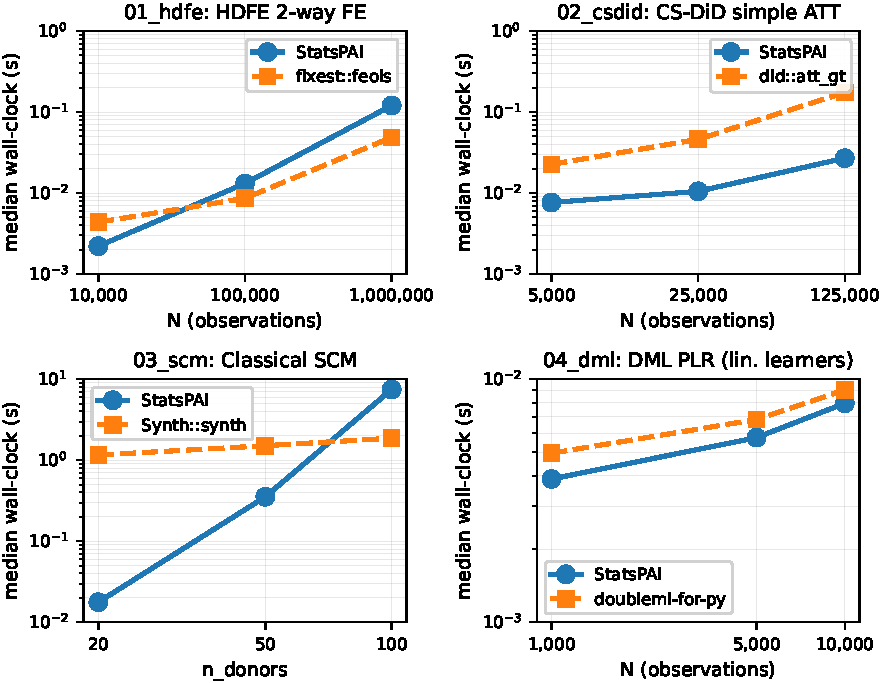
\includegraphics[width=\textwidth]{figures/track_c_loglog.pdf}
\caption{Log-log scaling of \statspai{} versus the declared reference
for the four Track-C benchmarks. The harness
runs both implementations on identical seed-fixed DGPs; points are
median wall-clock seconds across 3 or 5 reps after a warmup. Hardware:
Apple Silicon arm64 / 8 cores / 24~GB / macOS~26. The figure is
regenerated by \code{tests/perf/compare\_perf.py} on every benchmark
run.}
\label{fig:track-c-loglog}
\end{figure}

\paragraph{Reading the scaling figure.}
On the log-log axes of Figure~\ref{fig:track-c-loglog}, a roughly
constant vertical offset between two parallel lines is a constant-factor
runtime difference at matched asymptotic order, whereas a widening gap
(diverging slopes) signals a difference in computational complexity. The
figure shows whether each table gap is stable across the measured size
range or, as flagged below for classical SCM, grows with problem size
and therefore marks a genuine scaling target.

\paragraph{Headline findings.}
The results are mixed in the useful sense: they document where
\statspai{} is competitive and where the reference implementation is
still materially better.

\begin{itemize}[leftmargin=1.25em,itemsep=0.1em]
\item \textbf{HDFE 2-way FE}: at the largest measured row
($N = 10^6$), \pkg{fixest} is about $2.5\times$ faster than
\code{sp.fast.feols}. Both implementations remain sub-second at this
size, so the practical conclusion is parity of usable scale rather
than a \statspai{} speed win.
\item \textbf{Callaway--Sant'Anna staggered DiD}: \statspai{} is
about $6.5\times$ faster than \pkg{did} at $125{,}000$ observations
\emph{on the homogeneous-effect DGP used here}. The
homogeneous DGP is the cleanest case for the vectorized
group-time-ATT loop; on a heterogeneous-effect DGP with many treated
cohorts the gap should narrow because the IPW/DR cell-level
computation dominates on both sides; a heterogeneous-DGP
companion benchmark remains future work.
\item \textbf{DML PLR with linear nuisance learners}: \statspai{} and
\pkg{DoubleML} Python are effectively tied at the largest design
(\(0.008\) versus \(0.009\) seconds, ratio \(1.14\times\)). This
same-language comparison supports only the narrow conclusion that the
unified wrapper adds no material cost when nuisance fitting is cheap.
\item \textbf{Classical SCM}: \pkg{Synth} is about $4.0\times$ faster
than \statspai{} at $n_{\mathrm{donors}}=100$, while \statspai{} is the
faster of the two at 20 and 50 donors (Figure~\ref{fig:track-c-loglog}),
so the gap is one of scaling rather than fixed overhead. This is the main
performance gap exposed by Track~C. With more donors than
pre-treatment periods the inner weight problem is rank-deficient, so
each candidate \(V\) of the nested optimization is solved by
\pkg{scipy} SLSQP rather than the exact active-set solver used in the
full-rank case; that inner loop is the next optimization target.
\end{itemize}

\paragraph{Interpretation.}
The benchmark supports a modest claim: the package's unified surface
does not impose a productivity-prohibitive overhead for representative
workloads. One row favours \statspai{}, two favour the \proglang{R}
reference at the largest size, and the same-language DML row is tied.
It does not support a universal
``\proglang{Python} is faster'' claim. The SCM and HDFE rows are kept
in the table precisely because they are useful negative evidence for
future engineering priorities.

\section{Agent-facing interface checks}\label{sec:agentbench}

The agent-facing design described in Section~\ref{sec:agent} is the
most contestable claim in this paper: a reviewer may reasonably ask
whether a machine-readable schema \emph{actually} improves the
behaviour of an LLM agent on a real empirical task, or whether a
\emph{statsmodels-plus-prompting} baseline performs equivalently well.
That question needs frozen model releases, fixed prompts, matched tool
budgets, and a scoring rubric; it cannot be inferred from schema
coverage, and Section~\ref{sec:agentbench-behavioural} states what
answering it would take. The present section reports only the
\emph{mechanical} and \emph{contractual} evidence that the agent-facing
surface is correctly wired up. We refer to \citet{patil2023gorilla}
and \citet{liang2023helm} as methodological precedents for tool-use
and holistic-LLM benchmarks respectively.

\subsection{Mechanical evidence}\label{sec:agentbench-mechanical}

The function-schema layer is statically inspectable. We report in
Table~\ref{tab:schema-coverage} both the function-level coverage
($\RegistryTotal$ of $\RegistryTotal$ public functions emit a non-empty
OpenAI-style JSON Schema; \AgentCardCount{} currently expose curated or explicitly
inherited agent metadata cards) and the
parameter-level quality of those
schemas (\(\SchemaParameterTotal\) documented parameters across the
\(\RegistryTotal\) schemas, of which \(\SchemaParameterDefaultPct\) carry an
explicit default value and \(\SchemaParameterEnumPct\) carry enumerated
choices). Parameter quality
matters because the headline ``$\RegistryTotal/\RegistryTotal$ emit a schema'' figure is
high by construction -- the registry pipes \emph{any} typed signature
into a JSON Schema -- whereas the
stronger contract is that every parameter carries a
non-empty description. We do not turn
absence of package-distributed, package-wide OpenAI-style tool-schema catalogues
in \pkg{statsmodels}, \pkg{linearmodels}, or \pkg{scikit-learn} into
a numerical \emph{zero} score: those projects target different interfaces,
and Table~\ref{tab:schema-coverage} is an internal completeness audit,
not a behavioural or package-quality ranking; they do not rule out external
wrappers.

\begin{table}[t]
\centering\small
\begin{tabular}{@{}L{0.62\linewidth}rrr@{}}
\toprule
Audit item & Count & Missing & Share \\
\midrule
Public functions/classes                        & \RegistryTotal & --- & 100.0\% \\
Emit non-empty OpenAI-style tool schema          & \RegistryTotal & 0 & 100.0\% \\
Have at least one typed parameter                & \SchemaWithTypedParameter & --- & --- \\
Have non-empty function description              & \RegistryTotal & 0 & 100.0\% \\
Have curated or inherited agent metadata         & \AgentCardCount & \AgentDefaultCardCount & \AgentCardPct \\
\midrule
Parameters across all schemas                    & \SchemaParameterTotal & --- & 100.0\% \\
\quad with non-empty description                 & \SchemaParameterDescribed & 0 & \SchemaParameterDescribedPct \\
\quad with explicit default value                & \SchemaParameterDefault & --- & \SchemaParameterDefaultPct \\
\quad with enumerated choices (\code{enum})      & \SchemaParameterEnum & --- & \SchemaParameterEnumPct \\
\bottomrule
\end{tabular}
\caption{Internal mechanical schema audit for \statspai{} \StatsPAIVersion{}.
``Agent metadata'' means at least one non-empty assumption, pre-condition,
failure mode, limitation, or typical/minimum sample-size field after explicit
inheritance. The remaining schemas still emit name, signature, and
description fields, but are not counted as curated. Counts are regenerated
from the live registry; this table makes no cross-package quality claim.}
\label{tab:schema-coverage}
\end{table}

The same registry is exported as a versioned offline schema bundle
covering tool schemas, function schemas, agent cards, result-payload
validation, and provenance counts, so non-Python clients can discover
the tool surface without importing \statspai{}.

To keep this surface honest as the package grows, \statspai{} ships a
coverage ratchet for agent cards. The ratchet classifies registered
functions into cumulative documentation tiers, records per-field and
per-tier counters in a checked JSON floor, and fails CI on any
regression. The tiers deliberately separate a minimal schema-ready
description from richer assumptions, failure modes, alternatives, sample
size guidance, and certified/validated evidence. Lowering the floor
requires an explicit hand edit, so a schema-quality regression is
visible in code review rather than hidden behind a large function
count.

\subsection{Contractual trace evidence}\label{sec:agentbench-procedural}

The agent-facing surface is exposed through an MCP server
(Section~\ref{sec:mcp}) that negotiates Model Context Protocol
revisions 2024-11-05, 2025-03-26, and 2025-06-18. The protocol test
suite exercises the \code{initialize} handshake and version
negotiation, \code{tools/list} and \code{tools/call} with structured
content, and \code{isError} envelopes; the schema and registry suites
check that registered functions emit tool schemas, that agent-card
filters behave as documented, and that MCP tool discovery sees the same
registry-backed surface as \code{sp.function\_schema()}. These are the
package's own tests, not an external certification of protocol
conformance.

For this submission we also execute one deterministic end-to-end trace
through the live MCP server. The script
\code{replication/scripts/ex07\_agent\_trace.py} writes a temporary
\texttt{mpdta.csv} (the calibrated replica of Section~\ref{sec:ex-csdid},
so the traced estimate \(-0.0330\) is the replica value, not the
original-data \(-0.03995\)), calls \code{tools/list}, fits
\code{callaway\_santanna} with \code{as\_handle=true}, sends the
returned handle to \code{audit\_result}, and then sends the same
handle to \code{honest\_did\_from\_result}. It finally resolves the
returned citation keys through the MCP \code{bibtex} tool against the
curated \code{paper.bib}, so the trace exercises the citation
anti-hallucination contract rather than merely reporting key strings.
The same trace also sends a stale result-handle call to
\code{audit\_result} and checks that the MCP response is a recoverable
\code{isError} envelope with an actionable refit hint, so failure
recovery is exercised rather than only described.
Table~\ref{tab:agent-trace}
summarizes the trace; the normalized transcript is included in the
replication archive. The trace verifies the agent-specific claim that
the estimate \(\to\) audit \(\to\) sensitivity chain is executable
without ferrying arrays or hand-copying citations through the model
context.

\begin{table}[t]
\centering\small
\begin{tabular}{ll}
    \toprule
    Trace item & Value \\
    \midrule
    MCP tools listed & 559 \\
    Estimate & -0.0330 (SE 0.0078) \\
    Audit checks & 4 \\
    Honest-DiD max rejecting M & 0.0074 \\
    Recoverable stale-handle error & isError=True; hint present \\
    Verified citation keys & callaway2021difference, rambachan2023more \\
    BibTeX entries resolved & 2 \\
    \bottomrule
\end{tabular}

\caption{Deterministic MCP trace used for the agent-facing interface
check, including one recoverable stale-handle error path. Ephemeral
result handles are normalized in the transcript shipped with the
replication archive
(\code{replication/\allowbreak results/\allowbreak ex07\_agent\_trace.txt}).}
\label{tab:agent-trace}
\end{table}

\subsection{No behavioural benchmark claim}\label{sec:agentbench-behavioural}

Mechanical and contractual evidence does not answer whether an LLM agent
using this interface produces \emph{better empirical analyses} than one
using \pkg{statsmodels} or \proglang{R} packages through a Jupyter MCP
shim. That question requires frozen model
releases, fixed prompts, matched tool budgets, and a scoring rubric,
and belongs in a separate behavioural study. To make that deferral auditable
rather than vague, the archive includes
\code{replication/\allowbreak results/\allowbreak agent\_benchmark\_protocol.md}, which records
the matched arms, task families, scoring dimensions, leakage controls,
and minimum report items required before any behavioural claim is made.
The JSS contribution here is contractual: schemas, typed
errors, result handles, citations, and the deterministic trace are
reproducible interfaces, regenerated from the same validation ledger
that governs human-facing calls rather than from a separate
prompt-engineering layer, and they keep later benchmark scores from
being confounded with missing metadata or unverifiable citations.

\section{Computational details}\label{sec:compdetails}

\statspai{} installs from PyPI without compiled extensions of its own;
its numerical core runs on the scientific \proglang{Python} stack
(\pkg{numba}'s JIT compiler is the only compilation step, and it is
optional at runtime). The submitted artifact uses \proglang{Python}
3.12.1, \pkg{NumPy} 1.26.4,
\pkg{SciPy} 1.13.0, \pkg{pandas} 2.2.0, \pkg{statsmodels} 0.14.1,
\pkg{scikit-learn} 1.4.0, \pkg{linearmodels} 6.0, and
\pkg{matplotlib} 3.8 \citep{hunter2007matplotlib}. Optional heavy backends are isolated under extras
and are lazily imported. The submitted numerical and timing claims do
not require a compiled Rust extension, GPU, or commercial software.

The \proglang{R} parity harness is pinned by
\path{tests/r_parity/renv.lock}. The reference environment uses
\proglang{R} 4.5.2; the packages behind the twelve-estimator suite are
\pkg{fixest} 0.14.0, \pkg{did} 2.3.0,
\pkg{Synth} 1.1-10, \pkg{synthdid} 0.0.9, \pkg{rdrobust} 3.0.0,
\pkg{rddensity} 2.6, \pkg{HonestDiD} 0.2.8, \pkg{DoubleML} 1.0.2,
\pkg{grf} 2.6.1, and \pkg{MatchIt} 4.7.2, joined by \pkg{fect} 2.4.1
and \pkg{interflex} 1.4.0 for the three-ecosystem worked example; the
complete dependency closure for all \RParityModuleCount{} modules
(including \pkg{augsynth}, \pkg{gsynth}, \pkg{lme4}, \pkg{CBPS}
\citep{imai2014covariate}, \pkg{ebal} \citep{hainmueller2012entropy},
\pkg{optmatch} \citep{hansen2006optimal}, \pkg{Matching}
\citep{sekhon2011multivariate}, and \pkg{sbw}
\citep{wang2020minimal}) is recorded
with exact versions and GitHub SHAs in the lockfile and per-row JSON
provenance. The Stata bridge uses \proglang{Stata} 18 MP and records
official/community command versions in
\path{tests/stata_parity/STATA_ENVIRONMENT.md}. All \StataParityModuleCount{} R-joined Stata
modules and all \RParityModuleCount{} \proglang{R} modules reproduce their frozen JSON
outputs with zero drift; the Stata leg requires a licence, so the
archive ships the frozen JSONs, matching do-files, and engine
provenance, and the main paper remains auditable from the
\proglang{Python}/\proglang{R} artifacts.

\subsection{Distribution and installation}

The package is distributed through PyPI
(\code{pip install statspai}); this article describes release \StatsPAIVersion{}
(tag \code{v\StatsPAIVersion{}}). Optional extras are exposed as
\code{dev}, \code{performance}, \code{bayes}, \code{deepiv},
\code{neural}, \code{fixest}, \code{rd-cct}, and \code{plotting}
bundles. The \code{rd-cct} extra installs the official \pkg{rdrobust}
\proglang{Python} port (\code{rdrobust>=2.0}, maintained by the
\pkg{rdrobust} authors), which backs the optional \code{bwselect="cct"}
path of Section~\ref{sec:ex-rd}; that port is GPL-3 licensed, which is
why it is an opt-in extra installed by the user rather than a bundled
dependency of the MIT-licensed core. No parity claim in this paper
depends on it: the native default selector reproduces its numbers on
the audited fixture without it.

The test suite runs on Linux, macOS, and Windows in continuous
integration; the acceptance evidence for this paper is the Track~A--D
artifacts, worked examples, and audit scripts, each regenerated rather
than quoted.

\subsection{Reproducibility of this paper}\label{sec:reproducibility}

Reviewers can rebuild the paper's evidence along three paths, driven by
one standalone script, \path{Paper-JSS/replication/reproduce.py}. The
\emph{licence-free path} (\code{--tier 1}; the default) needs only the
pinned \proglang{Python} environment and runs in under ten minutes on
commodity hardware, inside the JSS one-hour threshold for a reviewer
verification path. It is important to be precise about what it does.
It \emph{recomputes} the seven worked examples, every manuscript listing
and transcript, the known-truth recovery tests, the seed-replicated
forest analysis, and the configuration map; it only \emph{re-derives
tables} from frozen artifacts for the three experiments that cost hours
--- Track~A parity, Track~B Monte Carlo, and Track~C timing. Each of
those has a separate, documented recomputation entry point
(Table~\ref{tab:reproduction}). The \emph{\proglang{R} path} (\code{--tier 2}) adds the
pinned \code{renv} environment and re-executes the cross-language
parity modules themselves, which the licence-free path can only replay
from frozen artifacts; by construction the paper's parity claim is a
comparison against \proglang{R}, so auditing the rows at full strength
requires this path. The \emph{\proglang{Stata} path} (\code{--tier 3})
re-executes the migration bridges and requires a Stata licence. A
Dockerfile reproduces the licence-free environment exactly.

Two further checks are on the paper rather than the package. The
listing audit replays each printed transcript statement by statement and
compares the printed output line for line with what the code produces.
And both sides of every parity row are re-derivable:
\path{tests/r_parity/verify_reproduce.py} re-runs each \proglang{R}
reference on the committed bytes, and
\path{tests/r_parity/verify_reproduce_py.py} does the same for the
\statspai{} side and also regenerates each fixture CSV byte for byte;
all \RParityModuleCount{} modules clear a \(10^{-9}\) reproduction
floor with no exemptions. On the licence-free path the parity,
coverage, and timing experiments are frozen evidence on that path;
Table~\ref{tab:reproduction} lists how to recompute each.

\begin{table}[!ht]
\centering\scriptsize
\begin{tabular}{@{}L{0.19\linewidth}L{0.15\linewidth}L{0.30\linewidth}L{0.13\linewidth}L{0.11\linewidth}@{}}
\toprule
Artifact & Tier~1 does & Full recomputation & Needs & Time \\
\midrule
Worked examples, listings (Sec.~\ref{sec:examples}) & recomputes & \code{reproduce.py} (Tier~1) & \proglang{Python} & \(<\)10 min \\
Track~A, \statspai{} side (Tab.~\ref{tab:track-a-parity}) & re-reads JSON & \code{--recompute parity-py} (and fixture bytes) & \proglang{Python} & \(\sim\)15 min \\
Track~A, \proglang{R} side & re-reads JSON & \code{--tier 2} & \proglang{R} 4.5.2, \code{renv.lock} & 30--60 min \\
Track~A, \proglang{Stata} side & re-reads JSON & \code{--tier 3} & \proglang{Stata} 18 & \(\sim\)30 min \\
Forest seeds (Tab.~\ref{tab:forest-seed-mc}) & re-analyses frozen draws & \code{--recompute forest-seed} & \proglang{Python}; \proglang{R} for \pkg{grf} side & \(\sim\)30 min + \(\sim\)20 min \\
Track~B (Tabs.~\ref{tab:track-b-b1000}--\ref{tab:track-b-robustness}) & re-reads JSON & \code{--recompute montecarlo} & \proglang{Python} & \(\sim\)80 min \\
Track~C (Fig.~\ref{fig:track-c-loglog}) & re-reads JSON & \code{--recompute performance} & \proglang{Python}; \proglang{R} for reference legs & hardware-dependent \\
\bottomrule
\end{tabular}
\caption{What the licence-free path recomputes and how to recompute the
rest (options of \code{replication/reproduce.py}); each writes to the
artifact path the paper reads.}
\label{tab:reproduction}
\end{table} The replication archive contains the
manuscript sources, replication scripts, selected package
source, validation tests, R/Stata/reference parity artifacts, Monte
Carlo and performance artifacts, and the deterministic MCP trace, and
fits within the JSS attachment limit.

\section{Discussion}\label{sec:discussion}

\statspai{} is a unification and validation project, not a new-estimator
paper. The claim is that a single \proglang{Python} package can expose
the applied causal workflow through shared result surfaces, explicit
validation status, reproducible parity artifacts, and machine-readable
agent schemas. It is not a claim that \statspai{} dominates specialized
reference packages in their home domains, nor that the MCP interface
replaces empirical judgement.

The main limitations are as follows. First, \RegistryAutoUnbacked{} stable auto-registered symbols remain API-stable but not parity-backed
(\RegistryAutoUnbackedClasslike{} class-like, \RegistryAutoUnbackedFunctionlike{} function-like), and the other \RegistryOtherApiEvidence{} symbols of the
\RegistryApiStable-symbol \code{api\_stable} tier carry API, unit-contract,
convention, or supplemental evidence only. The validated claim is
limited to certified/validated entries and to the named rows and modules in the validation-suite evidence; the validation-evidence
audit lists nine scoped limitation rows, each tied to a named function, evidence grade, and unsupported variant.
Second, only one Track~A row remains a methodological/T4 disclosure:
classical SCM on the calibrated Basque replica, where reference
implementations choose measurably different local optima; on the
original \code{Synth::basque} bytes the same specification brings all
three implementations within \(4\times10^{-4}\)
(Section~\ref{sec:scm-identification}), so the disclosure is about
data-dependent non-uniqueness, not a standing numerical defect. The
causal-forest row is T3: the two forest engines are equivalent to
within a tenth of a sampling standard error and equally noisy across
seeds, which is an equivalence claim, not parity. The
\ParityThirdPartyModuleCount{} Track~A rows served by third-party
\proglang{Python} libraries validate \statspai{}'s wrappers of those
libraries, not native algorithms. The configuration map behind
\code{sp.validation\_scope} covers the twelve suite estimators; for
the rest of the registry the evidence notes name the artifact but not
its configuration. Third,
the \pkg{fect} and \pkg{interflex} cross-validation selectors for the
factor number, penalty, and kernel bandwidth are ported in
1.29.0 but can only be graded T3: their folds are random,
so the three-ecosystem parity of Section~\ref{sec:ex-fect} is
established at user-specified tuning values, and the selectors are
checked by given-fold score equality plus across-seed agreement of the
selection. Fourth, Stata reproduction requires a
separate licence, so Stata rows are migration bridges rather than the
licence-free core of the archive; \NoStataModuleCount{} of the \RParityModuleCount{} modules carry no Stata
reference, each with a measured reason. Fifth, Bayesian, causal-discovery,
and behavioural-agent evaluations require different loss functions and
are outside this software-validation article. Sixth, within DiD, \statspai{} implements the apparatus of the
\citet{baker2026difference} practitioner's guide but not the efficient
combination of comparison groups and baseline periods
\citep{chen2025efficient} or selection-based pre-trend diagnostics
\citep{ghanem2026selection}.

The unification itself has costs worth stating plainly, because they
are the price of the design rather than defects of it. A unified API
necessarily lags its upstream references: when \pkg{did} or
\pkg{fixest} ships a new option, \statspai{} users wait for the ported,
parity-tested version, and the validation regime that makes the port
trustworthy is exactly what makes it slower to ship. The registry's
own census quantifies a second cost: \RegistryAutoUnbacked{} of the
registered symbols carry API-contract evidence only, so a user who
strays from the validated core onto a long-tail helper is relying on
software-engineering guarantees, not statistical validation -- which is
why the tier is printed at call time rather than in an appendix.
Third, the evidence regime itself has a maintenance bill: every
correctness fix in Table~\ref{tab:correctness-history} exists because a
parity or coverage artifact flagged it, and keeping \RParityModuleCount{}
modules pinned against two external ecosystems is ongoing work that a
single-method package does not carry.

A fourth cost is a limit of the regime rather than of the package. A
parity ledger validates the paths it exercises and is silent about the
rest: the 1.25.0 entry of Table~\ref{tab:correctness-history}, a
continuous-treatment forest path no Track~A or Track~B row reaches,
surfaced only in a worked example. That is why the registry records
\emph{which} artifact backs a label, why \code{sp.validation\_scope}
reports the configuration an artifact exercised, and why the worked
examples are executed end-to-end.

The roadmap is to resolve or further bound the remaining
classical-SCM reference-disagreement disclosure, extend
\(B=1{,}000\) coverage beyond the headline rows, close the two measured
performance gaps of Section~\ref{sec:performance}, and move the agent
interface from mechanical conformance to scored behavioural
benchmarking.

A final limitation is institutional: a large surface is maintained by a
small team with one principal author. The risk is bounded by
properties verifiable from the archive: the package is MIT-licensed with
no relicensing clause, so the validated core can be forked; every
output-changing fix is pinned by a regression test; and the parity
harness is scripted and environment-pinned (\code{renv.lock}, recorded
Stata versions, per-row JSON provenance), so any third party with the
reference runtimes can re-execute it.

\section*{Author contributions}

B.\,W.\ designed and implemented \statspai{}, the validation harnesses
and registry API, and drafted the manuscript. S.\,R.\ supervised the
applied-econometrics programme, advised on scope and validation priorities,
and reviewed the manuscript. Both authors approved the final version.

\section*{Acknowledgements}

The authors thank Stanford REAP for institutional support and feedback,
and the maintainers of the \proglang{Python}, \proglang{R}, and
\proglang{Stata} packages used as parity references. Any remaining
errors are the authors' own.

\section*{Conflict of interest}

\statspai{} is MIT-licensed open-source software. The authors are
affiliated with StatsPAI Inc., which maintains the package; CoPaper.AI
is a commercial downstream product that may call \statspai{} but is not
required to use it. B.\,W.\ is the creator and principal maintainer. No
external funder had a role in the validation studies, analysis, or
manuscript preparation.

\section*{AI usage disclosure}

Portions of code documentation and manuscript text were prepared with
large-language-model assistance. The authors selected the claims,
reviewed the text, and remain responsible for all statistical decisions.
Numerical claims are tied to tests, replication scripts, frozen JSON
artifacts, and cited references; citations are checked by the verifier
in Section~\ref{sec:cite}.


\bibliography{jss-bib}

\appendix

\section{The complete Track A ledger}\label{app:parity}

Table~\ref{tab:track-a-cross-language-snapshot} in Section~\ref{sec:track-a} prints a
twelve-row slice of Track A, chosen to span the validation suite. The
slice is a reading aid, not the evidence. The evidence is
Table~\ref{tab:track-a-parity} below: every one of the
\RParityModuleCount{} modules, with the worst residual gap each one
carries against its canonical \proglang{R} reference and, for
\StataParityModuleCount{} of them, against a canonical or audited
\proglang{Stata} bridge.

The difference columns are worst-case over each module's headline rows
and cover \emph{point estimates only}; every SE row of every passing
module is gated separately (Section~\ref{sec:adjudication}). The
parenthetical notes name the convention, delegation, or common
specification under which a row is claimed, and italic text in the
\proglang{Stata} column records a \emph{measured} reason that no
portable \proglang{Stata} artifact exists.

% AUTO-GENERATED by replication/scripts/gen_appendix_parity.py
% Data rows come from tests/r_parity/compare.py; the caption and
% table frame are authored in this script. Do not edit by hand.
\begingroup
\footnotesize
\setlength{\tabcolsep}{2pt}
\setlength{\LTcapwidth}{\linewidth}
\begin{longtable}{@{}L{0.045\linewidth}L{0.20\linewidth}L{0.305\linewidth}L{0.305\linewidth}L{0.075\linewidth}@{}}
\toprule
ID & Method & Worst diff vs \proglang{R} & Worst diff vs \proglang{Stata} & Verdict \\
\midrule
\endfirsthead
\multicolumn{5}{c}{\textit{(Table \ref{tab:track-a-parity} continued)}}\\
\toprule
ID & Method & Worst diff vs \proglang{R} & Worst diff vs \proglang{Stata} & Verdict \\
\midrule
\endhead
\midrule
\multicolumn{5}{r}{\textit{(continued on the next page)}}\\
\endfoot
\bottomrule
\caption{Every Track A module, at \statspai{}~\StatsPAIVersion{}.
The \code{ID} column is the module's two-digit prefix in
\code{tests/r\_parity/}. The two difference columns report the worst
residual gap across that module's headline rows, point estimates only;
per-row standard errors, confidence bounds, and documented convention
gaps are in the generated
\code{tests/r\_parity/results/parity\_table\_3way.md}. Italic text in
the \proglang{Stata} column is the measured reason no portable
\proglang{Stata} artifact exists for that module, not an untested
assumption of unavailability. All \RParityModuleCount{} modules are
joined to a canonical \proglang{R} reference and
\StataParityModuleCount{} additionally to a canonical or audited
\proglang{Stata} bridge, every side reading the same CSV bytes.}
\label{tab:track-a-parity}\\
\endlastfoot
\code{01} & OLS + HC1 SE & rel $\le \ensuremath{1.1\times 10^{-12}}$ & rel $\le \ensuremath{1.3\times 10^{-12}}$ & \textbf{PASS} \\
\code{02} & 2SLS + HC1 SE & rel $\le \ensuremath{1.1\times 10^{-11}}$ & rel $\le \ensuremath{1.1\times 10^{-11}}$ & \textbf{PASS} \\
\code{03} & HDFE 2-way FE & rel $\le \ensuremath{5.2\times 10^{-15}}$ {\footnotesize (fixest/reghdfe small-sample correction)} & rel $\le \ensuremath{2.9\times 10^{-15}}$ & \textbf{PASS} \\
\code{04} & CS-DiD simple ATT & rel $\le \ensuremath{1.3\times 10^{-15}}$ {\footnotesize (estimate and SE both rel $<$ \ensuremath{1\times 10^{-9}})} & rel $\le \ensuremath{1.3\times 10^{-15}}$ & \textbf{PASS} \\
\code{05} & Sun--Abraham event study & rel $\le \ensuremath{2.8\times 10^{-11}}$ {\footnotesize (fixest agg='att' summary parity)} & rel $\le \ensuremath{2.7\times 10^{-11}}$ & \textbf{PASS} \\
\code{06} & RD CCT bias-corrected & rel $\le \ensuremath{5.7\times 10^{-14}}$ {\footnotesize (native CCT default-$h$; official Py port recorded separately)} & rel $\le \ensuremath{9.4\times 10^{-11}}$ & \textbf{PASS} \\
\code{07} & Classical SCM & rel $\le 0.024$ {\footnotesize (T4 reference disagreement: native tracks Stata; R Synth differs; exact recovery on identified DGP \code{52})} & rel $\le 0.00042$ & \textit{GAP} \\
\code{08} & DML PLR (LinReg learners) & rel $\le 0$ {\footnotesize (shared explicit fold\_id)} & rel $\le \ensuremath{3.7\times 10^{-15}}$ & \textbf{PASS} \\
\code{09} & RD density (CJM) & rel $\le \ensuremath{9.3\times 10^{-12}}$ {\footnotesize (native CJM/rddensity default parity)} & rel $\le \ensuremath{1.8\times 10^{-11}}$ & \textbf{PASS} \\
\code{10} & Honest DiD bounds & abs $\le \ensuremath{1.41\times 10^{-8}}$ {\footnotesize (native FLCI; vs HonestDiD with exact quantile, and closed form at M=0; shipped HonestDiD's simulated quantile shown separately)} & abs $\le \ensuremath{9.38\times 10^{-9}}$ & \textbf{PASS} \\
\code{11} & PSM 1:1 NN & rel $\le \ensuremath{1.2\times 10^{-15}}$ {\footnotesize (se\_teffects\_ai joins Stata teffects psmatch's Abadie-Imbens 2016 estimated-score variance at rel \ensuremath{7\times 10^{-8}} via the abadie\_imbens\_2016 SE option; the default psmatch2 ai(1) SE is a documented convention (sample vs population ATT, no score term))} & rel $\le \ensuremath{2\times 10^{-16}}$ & \textbf{PASS} \\
\code{12} & Synthetic DID & rel $\le \ensuremath{7.8\times 10^{-16}}$ {\footnotesize (native Frank-Wolfe/zeta ATT parity; backend-native placebo SE diagnostics)} & rel $\le \ensuremath{7.2\times 10^{-8}}$ & \textbf{PASS} \\
\code{13} & Causal forest (AIPW) & rel $\le 0.00026$ {\footnotesize (T3; single draw per engine, graded by seed-replicated equivalence within 0.1 sampling SE)} & \emph{bridge artifact not materialized: Stata 19's official cate command is the candidate causal-forest/AIPW reference, but the verified local runtime is Stata 18 and `which cate` fails.} & \textbf{PASS} \\
\code{14} & OLS + cluster-robust SE & rel $\le \ensuremath{3\times 10^{-14}}$ & rel $\le \ensuremath{2.2\times 10^{-14}}$ & \textbf{PASS} \\
\code{15} & HDFE + cluster SE & rel $\le \ensuremath{5.2\times 10^{-15}}$ {\footnotesize (fixest/reghdfe nested-FE cluster correction)} & rel $\le \ensuremath{2.9\times 10^{-15}}$ & \textbf{PASS} \\
\code{16} & BJS imputation & rel $\le \ensuremath{4.8\times 10^{-8}}$ {\footnotesize (R/Stata simple-ATT point parity; SE rows side-specific)} & rel $\le \ensuremath{3.5\times 10^{-7}}$ & \textbf{PASS} \\
\code{17} & Wooldridge ETWFE & rel $\le \ensuremath{1.8\times 10^{-13}}$ {\footnotesize (emfx aggregation and cluster SE matched)} & rel $\le \ensuremath{3.9\times 10^{-14}}$ & \textbf{PASS} \\
\code{18} & Augmented SCM & rel $\le \ensuremath{7.9\times 10^{-6}}$ {\footnotesize (native centered Ridge+SCM parity; backend='augsynth' is a migration bridge)} & rel $\le \ensuremath{1.7\times 10^{-8}}$ & \textbf{PASS} \\
\code{19} & Generalized SCM (Xu 2017) & rel $\le \ensuremath{7.7\times 10^{-14}}$ {\footnotesize (native gsynth/fect two-way FE factor convention parity)} & rel $\le \ensuremath{2.2\times 10^{-15}}$ & \textbf{PASS} \\
\code{20} & Goodman--Bacon decomposition & rel $\le \ensuremath{5.6\times 10^{-16}}$ {\footnotesize (R/Stata bacondecomp dyad parity)} & rel $\le \ensuremath{9.6\times 10^{-9}}$ & \textbf{PASS} \\
\code{21} & Honest-DiD relative-mags & abs $\le \ensuremath{4.44\times 10^{-16}}$ {\footnotesize (native ARP conditional set; identical grid points)} & abs $\le \ensuremath{5.55\times 10^{-17}}$ & \textbf{PASS} \\
\code{22} & sensemakr robustness & rel $\le \ensuremath{5\times 10^{-8}}$ {\footnotesize (sensemakr RV and benchmark bound-scale parity)} & rel $\le \ensuremath{5\times 10^{-8}}$ & \textbf{PASS} \\
\code{23} & E-value (closed form) & rel $\le \ensuremath{5.8\times 10^{-14}}$ & rel $\le \ensuremath{1.2\times 10^{-16}}$ & \textbf{PASS} \\
\code{24} & Cox proportional hazards & rel $\le \ensuremath{8.4\times 10^{-16}}$ & rel $\le \ensuremath{2.1\times 10^{-10}}$ & \textbf{PASS} \\
\code{25} & Linear mixed model & rel $\le \ensuremath{2.6\times 10^{-12}}$ & rel $\le \ensuremath{8.3\times 10^{-11}}$ & \textbf{PASS} \\
\code{26} & GLMM logit (Laplace) & rel $\le 0.00017$ & rel $\le \ensuremath{1.4\times 10^{-8}}$ & \textbf{PASS} \\
\code{27} & GLMM logit (AGHQ, n=8) & rel $\le \ensuremath{1.7\times 10^{-7}}$ {\footnotesize (same 8-point AGQ likelihood (logLik rel \ensuremath{1\times 10^{-13}}); intercept within reference optimiser scatter on a flat objective)} & rel $\le \ensuremath{9.8\times 10^{-7}}$ & \textbf{PASS} \\
\code{28} & Stochastic frontier (cross-sec.) & rel $\le \ensuremath{4.1\times 10^{-8}}$ & rel $\le \ensuremath{4\times 10^{-8}}$ & \textbf{PASS} \\
\code{29} & Panel SFA (Pitt--Lee) & rel $\le \ensuremath{2.8\times 10^{-6}}$ {\footnotesize (slope parity; intercept/sigma rows are scale diagnostics)} & rel $\le \ensuremath{1.8\times 10^{-6}}$ & \textbf{PASS} \\
\code{30} & Blinder--Oaxaca decomposition & rel $\le \ensuremath{6.3\times 10^{-16}}$ {\footnotesize (twofold vs threefold split convention)} & rel $\le \ensuremath{1.3\times 10^{-16}}$ & \textbf{PASS} \\
\code{31} & DFL reweighting & rel $\le \ensuremath{1.2\times 10^{-9}}$ & rel $\le \ensuremath{1.8\times 10^{-13}}$ & \textbf{PASS} \\
\code{32} & RIF / UQR (median) & rel $\le \ensuremath{2.2\times 10^{-15}}$ & rel $\le \ensuremath{1.4\times 10^{-16}}$ & \textbf{PASS} \\
\code{33} & VAR (vars::VAR) & rel $\le \ensuremath{3.1\times 10^{-15}}$ & rel $\le \ensuremath{6.6\times 10^{-15}}$ & \textbf{PASS} \\
\code{34} & Local projections & rel $\le \ensuremath{5\times 10^{-15}}$ {\footnotesize (lpirfs Cholesky/unit-shock path (py-R) plus the direct-OLS Jorda regression (3-way); SEs are not joined on the direct rows because sp.local\_projections applies Newey-West while lm/regress report classical OLS)} & rel $\le \ensuremath{4.4\times 10^{-15}}$ & \textbf{PASS} \\
\code{35} & Panel FE/RE + Hausman$^{\dagger}$ & rel $\le \ensuremath{4.7\times 10^{-14}}$ {\footnotesize (FE/RE and plm-style Hausman parity; Stata sigmamore diagnostic row)} & rel $\le \ensuremath{1.5\times 10^{-15}}$ & \textbf{PASS} \\
\code{36} & Causal mediation (IKT) & rel $\le \ensuremath{6.7\times 10^{-15}}$ & rel $\le \ensuremath{3.6\times 10^{-15}}$ & \textbf{PASS} \\
\code{37} & PPML + HDFE & rel $\le \ensuremath{4.9\times 10^{-13}}$ {\footnotesize (post PPML FE-score fix; robust SE within 0.5\% of fixest)} & rel $\le \ensuremath{2.2\times 10^{-15}}$ & \textbf{PASS} \\
\code{38} & DR-DID (SZ 2020) & rel $\le \ensuremath{2.6\times 10^{-15}}$ {\footnotesize (panel DR-DID calibrated propensity parity with R/Stata)} & rel $\le \ensuremath{2.2\times 10^{-16}}$ & \textbf{PASS} \\
\code{39} & ARIMA(2,0,0)$^{\dagger}$ & rel $\le \ensuremath{7.4\times 10^{-7}}$ {\footnotesize (stats::arima ML / tightly converged Stata arima)} & rel $\le \ensuremath{9.3\times 10^{-9}}$ & \textbf{PASS} \\
\code{40} & Quantile reg (median) & rel $\le \ensuremath{3.3\times 10^{-15}}$ {\footnotesize (post sqrt(n) sandwich-scaling fix)} & rel $\le \ensuremath{4.4\times 10^{-15}}$ & \textbf{PASS} \\
\code{41} & Tobit (left-censored) & rel $\le \ensuremath{2.8\times 10^{-8}}$ {\footnotesize (post observed-information Hessian fix)} & rel $\le \ensuremath{2.8\times 10^{-8}}$ & \textbf{PASS} \\
\code{42} & Negative binomial & rel $\le \ensuremath{5.1\times 10^{-10}}$ & rel $\le \ensuremath{1\times 10^{-11}}$ & \textbf{PASS} \\
\code{43} & Heckman 2-step & rel $\le \ensuremath{1\times 10^{-11}}$ & rel $\le \ensuremath{1\times 10^{-11}}$ & \textbf{PASS} \\
\code{44} & Multinomial logit & rel $\le \ensuremath{2.6\times 10^{-7}}$ {\footnotesize (post observed-information Hessian fix)} & rel $\le \ensuremath{1.5\times 10^{-11}}$ & \textbf{PASS} \\
\code{45} & Ordered logit & rel $\le \ensuremath{1.5\times 10^{-7}}$ {\footnotesize (post observed-information Hessian fix)} & rel $\le \ensuremath{3.4\times 10^{-7}}$ & \textbf{PASS} \\
\code{46} & Conditional logit & rel $\le \ensuremath{1.3\times 10^{-8}}$ & rel $\le \ensuremath{1.3\times 10^{-8}}$ & \textbf{PASS} \\
\code{47} & PPML + 3-way HDFE & rel $\le \ensuremath{1.2\times 10^{-15}}$ {\footnotesize (Post Gauss-Seidel multi-FE fix; sp matches at \ensuremath{1\times 10^{-15}})} & rel $\le \ensuremath{1.2\times 10^{-16}}$ & \textbf{PASS} \\
\code{48} & Binary probit & rel $\le \ensuremath{3.1\times 10^{-7}}$ & rel $\le \ensuremath{1.6\times 10^{-8}}$ & \textbf{PASS} \\
\code{49} & Ordered probit & rel $\le \ensuremath{3.7\times 10^{-7}}$ & rel $\le \ensuremath{2.1\times 10^{-10}}$ & \textbf{PASS} \\
\code{50} & Arellano-Bond GMM & rel $\le \ensuremath{9\times 10^{-16}}$ {\footnotesize (R/Stata dynamic-panel fixture; block-diagonal instruments and one-step GMM weights match)} & rel $\le \ensuremath{1.4\times 10^{-15}}$ & \textbf{PASS} \\
\code{51} & Newey-West HAC OLS & rel $\le \ensuremath{1.4\times 10^{-15}}$ {\footnotesize (post HAC sandwich sqrt(n) scaling fix)} & rel $\le \ensuremath{8.5\times 10^{-16}}$ & \textbf{PASS} \\
\code{52} & Classical SCM (unique solution) & rel $\le \ensuremath{7.8\times 10^{-8}}$ {\footnotesize (identified convex SCM; sp and Stata synth recover exact weights+gap)} & rel $\le \ensuremath{7.7\times 10^{-8}}$ & \textbf{PASS} \\
\code{53} & Cluster-robust CR2 / CR3 SE & abs $\le \ensuremath{1.84\times 10^{-8}}$ {\footnotesize (CR2 and analytic CR3 match clubSandwich)} & abs $\le \ensuremath{5.93\times 10^{-9}}$ & \textbf{PASS} \\
\code{54} & Two-way cluster-robust SE & abs $\le \ensuremath{7.84\times 10^{-16}}$ {\footnotesize (matches sandwich::vcovCL(HC1,cadjust); fixest min-G df convention differs $\sim10^{-3}$)} & abs $\le \ensuremath{1.33\times 10^{-15}}$ & \textbf{PASS} \\
\code{55} & HC2 / HC3 robust SE & abs $\le \ensuremath{6.39\times 10^{-9}}$ & abs $\le \ensuremath{4.01\times 10^{-13}}$ & \textbf{PASS} \\
\code{56} & Three-way cluster-robust SE & abs $\le \ensuremath{2.09\times 10^{-15}}$ & abs $\le \ensuremath{7.77\times 10^{-16}}$ & \textbf{PASS} \\
\code{57} & Binary logit ML & rel $\le \ensuremath{2.7\times 10^{-11}}$ & rel $\le \ensuremath{2.7\times 10^{-11}}$ & \textbf{PASS} \\
\code{58} & Poisson ML & rel $\le \ensuremath{9.2\times 10^{-15}}$ & rel $\le \ensuremath{8.7\times 10^{-12}}$ & \textbf{PASS} \\
\code{59} & LIML k-class IV & rel $\le \ensuremath{1.7\times 10^{-15}}$ {\footnotesize (ivregress runs with `small` (RSS/(n-k)))} & rel $\le \ensuremath{9.7\times 10^{-16}}$ & \textbf{PASS} \\
\code{60} & SUR one-step FGLS & rel $\le \ensuremath{1.5\times 10^{-14}}$ {\footnotesize (Sigma divisor n (sureg default / noDfCor))} & rel $\le \ensuremath{1.5\times 10^{-15}}$ & \textbf{PASS} \\
\code{61} & Beta regression ML & rel $\le \ensuremath{2.2\times 10^{-12}}$ {\footnotesize (betareg SEs are expected-information (documented))} & rel $\le \ensuremath{2.1\times 10^{-8}}$ & \textbf{PASS} \\
\code{62} & Truncated regression ML & rel $\le \ensuremath{3.5\times 10^{-10}}$ & rel $\le \ensuremath{7.9\times 10^{-8}}$ & \textbf{PASS} \\
\code{63} & Zero-inflated Poisson & rel $\le \ensuremath{1.2\times 10^{-7}}$ & rel $\le \ensuremath{2.8\times 10^{-8}}$ & \textbf{PASS} \\
\code{64} & Zero-inflated NB & rel $\le \ensuremath{9.5\times 10^{-7}}$ {\footnotesize (flat ZINB likelihood near optimum (\ensuremath{1\times 10^{-5}} budget))} & rel $\le \ensuremath{4.5\times 10^{-11}}$ & \textbf{PASS} \\
\code{65} & Spatial ML (SAR/SEM/SDM) & rel $\le \ensuremath{8.3\times 10^{-8}}$ {\footnotesize (vs spatialreg::lagsarlm/errorsarlm/Durbin, row-std rook W)} & rel $\le \ensuremath{5.1\times 10^{-8}}$ & \textbf{PASS} \\
\code{66} & Spatial GMM (SAR-2SLS/SEM-GMM) & rel $\le \ensuremath{4.6\times 10^{-8}}$ {\footnotesize (vs spatialreg::stsls(W2X=F)/GMerrorsar; SEM point-only)} & rel $\le \ensuremath{7.3\times 10^{-16}}$ & \textbf{PASS} \\
\code{67} & Panel GLM (feglm / fepois)$^{\dagger}$ & rel $\le \ensuremath{9.7\times 10^{-9}}$ {\footnotesize (vs fixest::feglm/fepois, absorbed id FE; IWLS SE \ensuremath{1\times 10^{-5}})} & rel $\le \ensuremath{1.8\times 10^{-9}}$ & \textbf{PASS} \\
\code{68} & Within transformation & rel $\le \ensuremath{3.5\times 10^{-15}}$ {\footnotesize (sp.demean(solver='map') vs textbook mean-within)} & rel $\le \ensuremath{8.8\times 10^{-15}}$ & \textbf{PASS} \\
\code{69} & Panel balance filter & rel $\le 0$ {\footnotesize (sp.balance\_panel vs base R counts == n\_periods)} & rel $\le 0$ & \textbf{PASS} \\
\code{70} & Policy tree (exact, depth 1--2) & rel $\le \ensuremath{9.6\times 10^{-16}}$ {\footnotesize (shared AIPW scores; exact welfare optimum vs policytree, all 1200 per-row policy decisions identical at both depths)} & rel $\le \ensuremath{1.4\times 10^{-16}}$ & \textbf{PASS} \\
\code{71} & DML family (IRM / PLIV / IIVM) & rel $\le \ensuremath{9.1\times 10^{-11}}$ {\footnotesize (shared explicit fold\_id across all three DoubleML model classes; PLIV at the floating-point floor, IRM/IIVM limited by the logistic-MLE optimiser)} & rel $\le \ensuremath{6.9\times 10^{-7}}$ & \textbf{PASS} \\
\code{72} & TMLE (targeting step) & rel $\le \ensuremath{1.9\times 10^{-9}}$ {\footnotesize (shared initial Q / g1W; per-arm fluctuation matching tmle::tmle's submodel)} & rel $\le \ensuremath{1.9\times 10^{-9}}$ & \textbf{PASS} \\
\code{73} & Gardner two-stage DiD & rel $\le \ensuremath{4.8\times 10^{-8}}$ {\footnotesize (estimate rel \ensuremath{4.8\times 10^{-8}} and SE rel \ensuremath{2.7\times 10^{-10}} against did2s (Stata did2s: \ensuremath{2.4\times 10^{-12}} / \ensuremath{1.3\times 10^{-14}}); vce='analytic' is the did2s corrected two-stage clustered variance, so stage-1 estimation error is propagated on all three sides)} & rel $\le \ensuremath{2.4\times 10^{-12}}$ & \textbf{PASS} \\
\code{74} & Changes-in-Changes (ATT + QTE) & rel $\le \ensuremath{2.4\times 10^{-15}}$ {\footnotesize (machine precision vs qte::CiC (worst \ensuremath{4.4\times 10^{-15}}))} & rel $\le 0.006$ {\footnotesize (Stata convention gap)} & \textbf{PASS} \\
\code{75} & Stacked DiD (never-treated controls) & rel $\le \ensuremath{3.9\times 10^{-13}}$ {\footnotesize (rel < \ensuremath{1\times 10^{-6}} vs a hand-written fixest stack)} & rel $\le \ensuremath{7.1\times 10^{-13}}$ & \textbf{PASS} \\
\code{76} & Pre-trends power (Roth 2022) & rel $\le \ensuremath{4\times 10^{-5}}$ {\footnotesize (rel < \ensuremath{1\times 10^{-4}} vs pretrends::pretrends; the \ensuremath{1\times 10^{-3}} budget covers mvtnorm::pmvnorm's randomised integrator)} & rel $\le 0.00014$ & \textbf{PASS} \\
\code{77} & Triple differences ATT(g,t) & rel $\le \ensuremath{5.7\times 10^{-15}}$ {\footnotesize (machine precision vs triplediff::ddd (worst \ensuremath{1\times 10^{-12}}), estimates and analytic SEs, across dr / ipw / reg)} & \emph{no Stata implementation: the Ortiz-Villavicencio/Sant'Anna DDD estimator ships as the R package triplediff. Re-checked 2026-08-06: neither `triplediff` nor `ddd` resolves locally and `ssc describe triplediff` returns r(601).} & \textbf{PASS} \\
\code{78} & dCDH intertemporal event study & rel $\le \ensuremath{3.3\times 10^{-15}}$ {\footnotesize (machine precision vs DIDmultiplegtDYN (worst \ensuremath{5\times 10^{-15}}), across absorbing and switch-off designs)} & rel $\le \ensuremath{2.1\times 10^{-15}}$ & \textbf{PASS} \\
\code{79} & Functional-form test (Roth--Sant'Anna) & rel $\le \ensuremath{1.3\times 10^{-14}}$ {\footnotesize (machine precision vs didFF (worst \ensuremath{1.2\times 10^{-15}}); the module's \ensuremath{1\times 10^{-3}} budget covers only the simulated p-value)} & \emph{no Stata implementation: the Roth-Sant'Anna functional-form test ships as the R package didFF (GitHub only, not CRAN). Re-checked 2026-08-06: `ssc describe didff` returns r(601), not found.} & \textbf{PASS} \\
\code{80} & Continuous-treatment DiD (CGS) & rel $\le \ensuremath{2.4\times 10^{-14}}$ {\footnotesize (machine precision vs contdid::cont\_did (worst \ensuremath{1\times 10^{-12}}))} & \emph{no Stata implementation: the CGS continuous-treatment estimator ships as the R package contdid (GitHub only, not CRAN). Re-checked 2026-08-06: `ssc describe contdid` returns r(601), not found.} & \textbf{PASS} \\
\code{81} & dCDH 2020 DID\_M (on/off switching) & rel $\le \ensuremath{3.9\times 10^{-15}}$ {\footnotesize (machine precision vs archived DIDmultiplegt 0.1.4)} & rel $\le \ensuremath{3.2\times 10^{-15}}$ & \textbf{PASS} \\
\code{82} & Design-based staggered rollout (Roth-Sant'Anna) & rel $\le \ensuremath{9.1\times 10^{-16}}$ {\footnotesize (machine precision on all 33 rows (worst \ensuremath{3.7\times 10^{-15}}) against both staggered 1.2.2 in R and the SSC staggered port in Stata, including both the Neyman and adjusted standard errors)} & rel $\le \ensuremath{5.7\times 10^{-16}}$ & \textbf{PASS} \\
\code{83} & LP-DiD event study (Dube-Girardi-Jorda-Taylor) & rel $\le \ensuremath{5\times 10^{-15}}$ {\footnotesize (estimate and SE both rel $<$ \ensuremath{1\times 10^{-14}} vs a direct transcription)} & rel $\le \ensuremath{2.5\times 10^{-15}}$ & \textbf{PASS} \\
\code{84} & BJS pre-treatment lead vector (Borusyak-Jaravel-Spiess) & rel $\le \ensuremath{5.1\times 10^{-8}}$ {\footnotesize (point estimates rel $<$ \ensuremath{1\times 10^{-7}} against both references; the three leads match Stata \texttt{pretrends(3)} at rel $<$ \ensuremath{1\times 10^{-14}} on estimate and SE, and are a py$\leftrightarrow$Stata pin because R exposes no equivalent option; horizon SEs are an open gap)} & rel $\le \ensuremath{5.1\times 10^{-10}}$ & \textbf{PASS} \\
\code{85} & Dynamic TWFE event study (benchmark specification) & rel $\le \ensuremath{3.2\times 10^{-13}}$ {\footnotesize (estimates three-way to \ensuremath{5.7\times 10^{-14}}; SE matches \code{fixest} to \ensuremath{9.3\times 10^{-14}} under \code{ssc(fixef.K="none")}, and \code{reghdfe}'s SE is reproduced from it by the exact $(N-K\_{py})/(N-K\_{St})$ d.f. scalar)} & rel $\le \ensuremath{1.5\times 10^{-14}}$ & \textbf{PASS} \\
\code{86} & fect counterfactual estimators (fe / ife / mc) & rel $\le \ensuremath{1.8\times 10^{-13}}$ {\footnotesize (native port of fect's EM map; three outcome models on one staggered panel)} & rel $\le \ensuremath{9.8\times 10^{-10}}$ & \textbf{PASS} \\
\code{87} & interflex marginal effects (linear / binning / kernel) & rel $\le \ensuremath{4\times 10^{-15}}$ {\footnotesize (native port incl. R's density() grid for the adaptive kernel bandwidth)} & rel $\le \ensuremath{1.5\times 10^{-14}}$ & \textbf{PASS} \\
\code{88} & RD bandwidth selection (all ten CCT selectors) & rel $\le \ensuremath{9.4\times 10^{-13}}$ {\footnotesize (all 68 bandwidths agree with \pkg{rdrobust} to \ensuremath{1.8\times 10^{-12}} and with Stata to \ensuremath{3.7\times 10^{-9}}; \code{certwo} is pinned against R only because Stata \code{rdbwselect} 10.0.0 exits \code{r(3200)} on that selector, including on the package authors' own \code{rdrobust\_senate.dta})} & rel $\le \ensuremath{3.5\times 10^{-9}}$ & \textbf{PASS} \\
\code{89} & Multi-score / geographic RD at boundary points & rel $\le \ensuremath{1.2\times 10^{-12}}$ {\footnotesize (three boundary points along one boundary; bias-corrected and conventional estimates, standard errors, selected bandwidths and per-side effective sample sizes agree with \pkg{rdmulti} to \ensuremath{7.6\times 10^{-12}} and with Stata to \ensuremath{3.3\times 10^{-9}}, and the six effective sample sizes are exactly equal on all three sides)} & rel $\le \ensuremath{5.4\times 10^{-10}}$ & \textbf{PASS} \\
\end{longtable}
\endgroup


\noindent Of the \RParityModuleCount{} modules, all but one receive a
pass-type verdict. A pass-type verdict covers ordinary strict passes,
common-specification passes such as RD at a forced common bandwidth,
seeded stochastic passes such as DML, and coefficient-level passes whose
secondary diagnostic follows a documented small-sample convention. The
single remaining \textit{GAP} is the classical-SCM donor-weight
non-uniqueness disclosure of
Section~\ref{sec:scm-identification}, kept visible rather than absorbed
into a wider tolerance.

Two things this table does not do: it omits per-row detail, which is
regenerated into \code{tests/r\_parity/results/parity\_table\_3way.md},
and it does not by itself show that either side is re-derivable
(Section~\ref{sec:reproducibility}).

\section{Output-changing corrections}\label{app:corrections}

Table~\ref{tab:correctness-history} lists the output-changing fixes that
affect interpretation of the present validation claim; each is pinned by
a regression test, and users on affected versions should re-estimate.
Section~\ref{sec:parity-gaps} discusses the 1.23.0 and 1.25.0 entries;
none of the 174 defects of 1.29.0 had been caught by a unit test.

\begin{table}[!ht]
\centering\scriptsize
\begin{tabular}{@{}p{0.08\linewidth}p{0.25\linewidth}p{0.61\linewidth}@{}}
\toprule
Version & Affected area & Output-changing fix \\
\midrule
1.6--1.15 & IV/LIML/Heckman, event study, CS-DiD, TMLE, DML, metalearners, mediation & Small-sample, two-step and rank SE corrections; influence-function, orthogonal-score and AIPW fixes. \\
1.16.0 & Quantile regression, Newey--West, Arellano--Bond; forest ATE/ATT & SE scaling and GMM weight construction corrected; forest headline moved to the \pkg{grf} AIPW estimand. \\
1.21.0 & CBPS, entropy balancing, Mahalanobis, genetic matching & GMM basis, exact moment balance, and covariance conventions corrected (up to $8.6\times$ off \pkg{CBPS}); now pinned against \pkg{CBPS}, \pkg{ebal}, \pkg{MatchIt}, \pkg{optmatch}, \pkg{Matching}, \pkg{sbw}. \\
1.23.0 & CS-DiD unit weights; IPW SEs & Weighted estimand restored; IPW SEs were 9--11\% (up to 89\% weighted) too large; pinned to \code{did::att\_gt} (see text). \\
1.24.0 & Sun--Abraham, GLMM, PPML-HDFE, dynamic TWFE SEs & Degrees-of-freedom/nesting conventions fixed to the reference rules; SEs moved 0.1--2\% (see text). \\
1.25.0 & Causal-forest aggregation under a continuous treatment & The binary AIPW score was applied to a continuous treatment ($-1266.6$, $p=0.0000$ on Card); guarded in 1.25.0, replaced by the Riesz-representer average in 1.29.0. Binary results unchanged. \\
1.26.0 & Evidence grades & A false alias certification (\code{sp.wooldridge\_did} as \code{sp.etwfe}) withdrawn; grades, not estimates, changed. \\
1.27.0 & ETWFE, \code{sp.wooldridge\_did}, \code{sp.etregress}, RE panel logit/probit, panel FGLS, spatial LM tests & Cohort ATTs read from a saturated regression; clustered SEs account for absorbed effects; the \code{etregress} default is a true MLE with first-stage-aware two-step SEs; \code{lm\_tests} no longer reverses its model-selection conclusion. \\
1.28.0 & SCM placebo \(p\)-values; Mendelian randomization; evidence grades & Permutation \(p\)-values now rank the treated unit with its placebos, \((1+\#\{\text{placebo}\ge\text{treated}\})/(J+1)\); MR estimators ported to their reference definitions; 31 functions graded T2 on closed-form tests that never ran \proglang{R} or \proglang{Stata} were regraded T1 (see text). \\
1.29.0 & Cross-language parity campaign (174 defects) and Track A closure & Fourteen families bisected against their reference on identical bytes; 174 output-changing defects fixed, none caught by a unit test; forest defaults follow \pkg{grf}; Gardner two-stage SE as \pkg{did2s}; PSM SE as \code{teffects psmatch}. \\
1.30.0 & HonestDiD on a raw CS fit; forest ATT/ATC under a continuous treatment & The event-study covariance passed to \code{sp.honest\_did} dropped the cohort-share term off the diagonal (cross-cell entries up to 8\% off \pkg{did}), overstating robustness; now matches \pkg{did} to \(2.8\times10^{-13}\), and the bounds of Listing~\ref{lst:csdid-output} moved in the fourth decimal. ATT and ATC now raise for a continuous treatment, as in \pkg{grf}. \\
1.31.0 & Entropy-balancing SE; audit applicability; Honest-DiD relative magnitudes; evidence grades & \code{sp.ebalance} SE was twice the Monte Carlo SD; now the M-estimation sandwich (\pkg{WeightIt} to \(3\times10^{-9}\)). \code{sp.audit}: over-identification test not applicable on just-identified fits. \code{sp.causal\_question} forest design reports the forest's own AIPW average. Native relative-magnitudes Honest-DiD set; two parity rows that ran \proglang{R} itself rebuilt on native code; forest T3 re-established by seed replication. \\
\bottomrule
\end{tabular}
\caption{Output-changing correctness fixes through release
\StatsPAIVersion{}; CHANGELOG and \code{MIGRATION.md} hold the detail.}
\label{tab:correctness-history}
\end{table}


\end{document}
